\documentclass[acmtog]{acmart}
\setcopyright{none}
\citestyle{acmauthoryear}
\settopmatter{printacmref=false,printccs=false,printfolios=true}
\renewcommand\footnotetextcopyrightpermission[1]{}
\usepackage[T1]{fontenc}
\usepackage[utf8]{inputenc}
\usepackage{textcomp}
\usepackage{amsmath}
\usepackage{booktabs,array,tabularx,multirow}
\usepackage{graphicx}
\usepackage{tikz}
\usepackage{xcolor}
\usepackage{microtype}
\usepackage{siunitx}
\usepackage{enumitem}
\usepackage{url}
\usepackage{bookmark}
\setlength{\emergencystretch}{3em}
\setlength{\textfloatsep}{9pt plus 2pt minus 2pt}
\setlength{\floatsep}{7pt plus 2pt minus 2pt}
\providecommand{\tightlist}{\setlength{\itemsep}{0pt}\setlength{\parskip}{0pt}}
\sisetup{round-mode=places,round-precision=3,detect-weight=true}
\hypersetup{hidelinks,pdftitle={Reality Probe: Verifying Physical Edits in Video-Reconstructed Worlds},pdfauthor={Swayam Singal}}
\title{Reality Probe: Verifying Physical Edits in Video-Reconstructed Worlds}
\author{Swayam Singal}
\email{swayam.singal@gmail.com}
\ccsdesc[500]{Computing methodologies~Physical simulation}
\ccsdesc[300]{Computing methodologies~Computer graphics}
\keywords{video-reconstructed worlds, physical editing, inverse physics, physical verification, uncertainty, experiment design, Gaussian splatting}
\begin{document}
\begin{abstract}
Video-based inverse physics can turn a recording into a model whose material or dynamic parameters are later edited and simulated. The dangerous case is simple: an optimizer changes a physical parameter because the new value matches held-out motion better, yet the edited model behaves less correctly under a different interaction. A fitting loss cannot tell the system whether that change should be committed. We introduce Reality Probe, a verification layer that evaluates a candidate physical edit using evidence withheld from fitting and returns SUPPORT, VETO, or UNRESOLVED. Across controlled and measured studies, verification succeeds or fails mainly with the information carried by the physical test: numerically sound contrasts can remain uninformative, while a better-matched intervention can separate candidate models. On a locked 10-video IRIS pendulum evaluation, a finite-amplitude probe raises decision accuracy from 36.4\% to 81.8\% over a small-angle baseline; a separately frozen free-fall protocol fails untouched validation and is retired. The practical consequence is architectural: physically editable scene systems should separate fitting from acceptance, and require physical evidence before a model change becomes part of the persistent world.
\end{abstract}

\maketitle
\pagestyle{plain}
\thispagestyle{plain}

\section{Introduction}\label{introduction}

Suppose a cloth has been reconstructed from video and assigned a simulated stiffness. A later optimization pass proposes a new stiffness because it lowers trajectory error on held-out frames. If the system simply overwrites the old value, it is treating better fit as evidence of better physics. Those are different claims. The new parameter may reproduce the recorded motion more closely and still respond worse when the cloth is pulled, struck, or loaded in a way that was never part of fitting.

This problem appears whenever a reconstructed scene is expected to remain physically editable. By a \emph{video-reconstructed world}, we mean a scene model recovered from observations that stores geometry or appearance together with state or parameters used by a simulator. Physics-aware radiance fields, Gaussian representations, and differentiable simulators increasingly support this combination of reconstruction, parameter estimation, and interaction synthesis \citep{li2023pacnerf,xie2024physgaussian,zhang2024physdreamer,liu2025physflow,rho2026monophysics,wada2026mphygs,hu2019chainqueen,hu2020difftaichi}. Once such a model persists beyond the fitting run, every physical parameter change becomes a state-management decision: should the system keep the old model or commit the new one?

Inverse physics usually answers a different question: which parameters best explain the observations used for estimation? Structural identifiability asks whether those observations can determine the parameters at all, and experiment design asks which measurements make competing models easier to distinguish \citep{wang2026identifiability,asadi2025oed}. Verification and validation ask whether a computational model is credible for an intended use \citep{oberkampf2007pcmm,laudy2026digitaltwin}. The missing systems step is the acceptance decision for one concrete physical edit after an optimizer has proposed it. A persistent scene needs a way to say: \emph{this change is physically supported}, \emph{this change is contradicted}, or \emph{the available test does not tell us enough}.

Reality Probe inserts that decision between proposal and commit. The candidate is produced from fitting data and ordinary held-out observations. After the candidate is fixed, a reserved physical observation or intervention is evaluated against both the baseline and the candidate. Measurement, repeat, and numerical uncertainty are carried into the comparison. The result is SUPPORT, VETO, or UNRESOLVED. SUPPORT permits a verified commit; VETO keeps the baseline because the candidate is physically worse on the reserved test; UNRESOLVED keeps the baseline because the experiment cannot separate the two models strongly enough.

Figure~\ref{fig:overview} shows the failure that motivates this gate. In one frozen synthetic example, the candidate improves ordinary held-out error by 14.93\% but worsens an untouched physical target by 9.03\%. The example is illustrative rather than statistically privileged. What matters is the structure of the failure: the metric used to choose the edit and the physical behavior we ultimately care about can move in opposite directions.

\begin{figure*}[t]
\centering
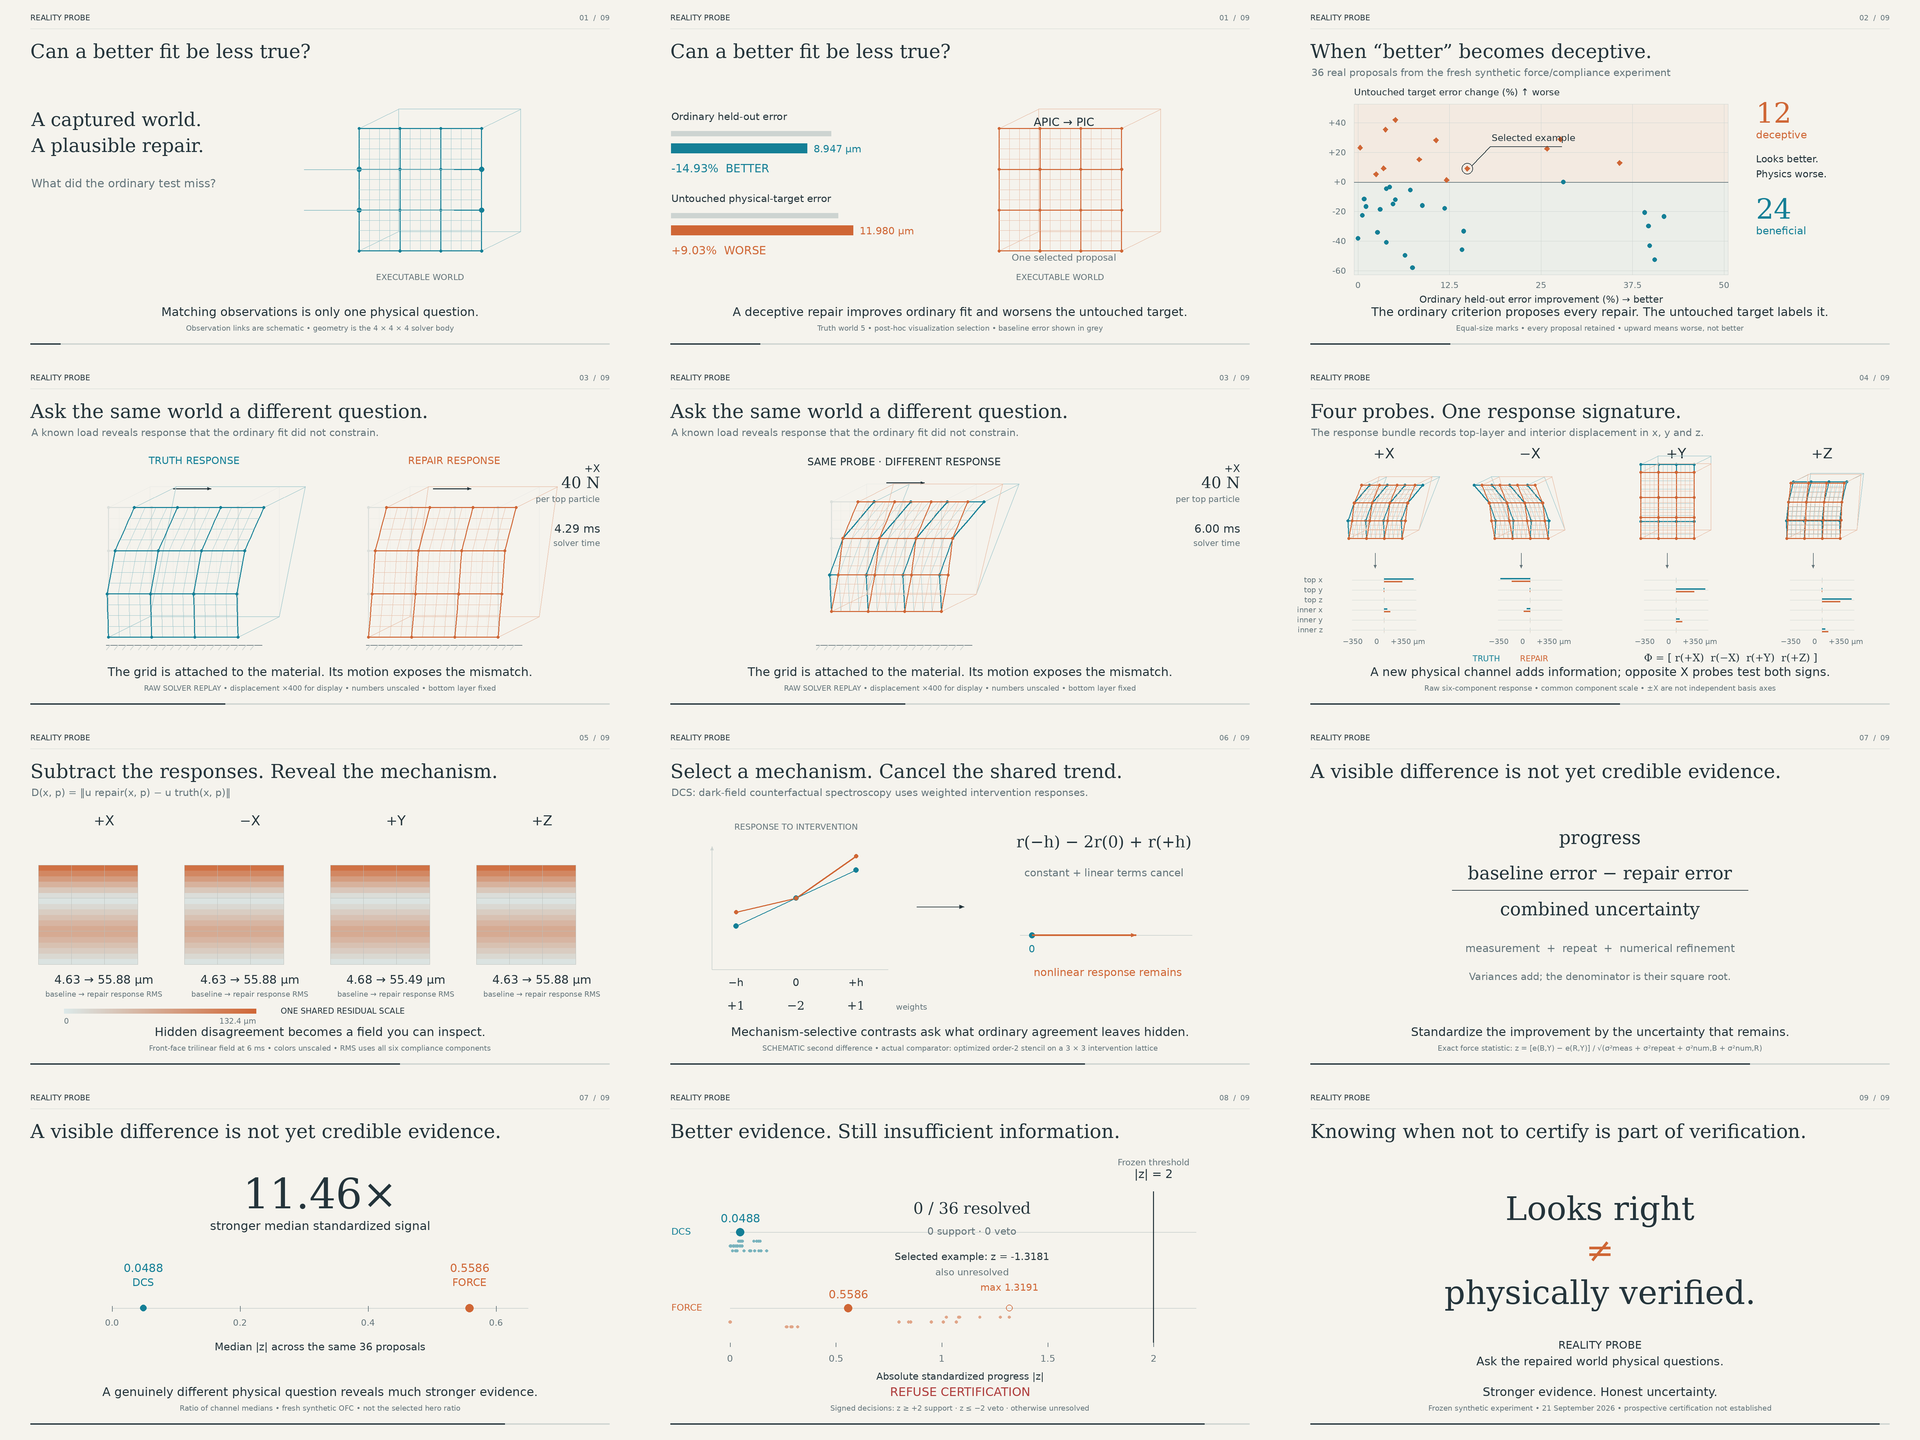
\includegraphics[width=\textwidth]{../docs/readme_assets/storyboard.png}
\caption{Reality Probe separates proposing a physical edit from accepting it. A candidate can improve ordinary held-out fit while degrading an untouched physical behavior. After the candidate is fixed, the system asks a reserved physical question, compares baseline and candidate responses under uncertainty, and either commits the candidate, vetoes it, or leaves the decision unresolved.}
\label{fig:overview}
\end{figure*}

\begin{figure}
\centering
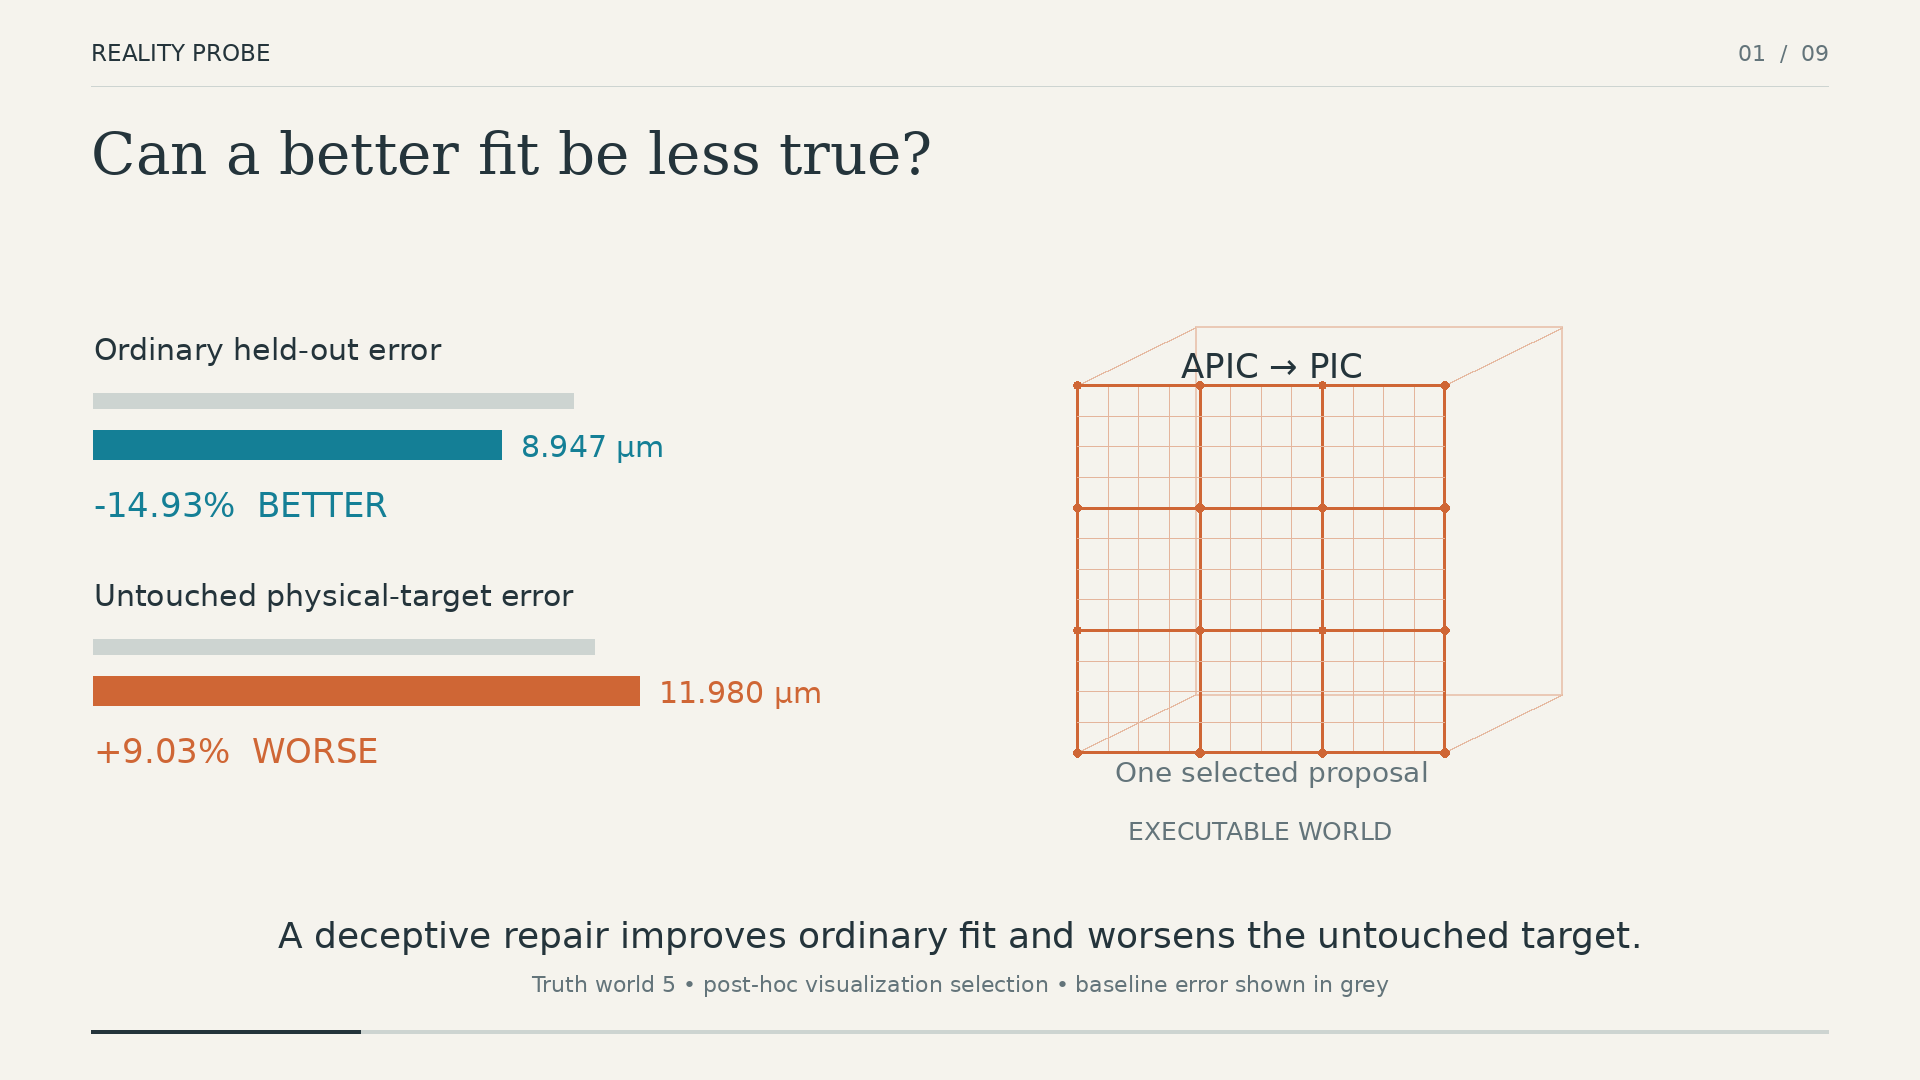
\includegraphics[width=\linewidth]{../docs/readme_assets/02_deceptive_repair.png}
\caption{Example of a fit-improving physical regression from the frozen synthetic population. Ordinary held-out error decreases by 14.93\%, while untouched-target error increases by 9.03\%. This case is shown for intuition and does not determine any threshold or aggregate result.}
\label{fig:deceptive-repair}
\end{figure}

The central hypothesis of this paper is not that one verifier works everywhere. It is that the usefulness of verification depends on whether the reserved physical test contains information that distinguishes the candidate from the baseline. We therefore evaluate several evidence channels rather than tuning one mechanism until it passes. Dark-Field Counterfactual Spectroscopy (DCS) tests whether signed intervention contrasts expose higher-order disagreement. Known-force compliance changes the physical question entirely. IRIS pendulum video provides a measured setting where a dynamics-matched observable succeeds. A separately frozen free-fall protocol provides a measured setting where the verification approach fails validation. The negative result is part of the contribution because it shows where the acceptance gate must refuse to generalize.

The impact is architectural. A physically editable scene should not be a fit-and-commit pipeline. It should be a \emph{fit, test, then commit} pipeline in which the acceptance evidence is distinguishable from the evidence that produced the candidate. This makes silent physical regressions observable and gives the system a principled reason to preserve the previous state when its experiment is uninformative.

The paper makes three contributions:

\begin{enumerate}
\def\labelenumi{\arabic{enumi}.}
\item
  \textbf{An evidence-gated commit model for physical scene edits.} Reality Probe separates proposal data from acceptance data, propagates the uncertainty of the reserved test, and records SUPPORT, VETO, or UNRESOLVED before a candidate physical state can replace the baseline.
\item
  \textbf{An empirical study of verification information.} Controlled synthetic experiments show that mathematically valid and numerically stable probes can remain too weak to support a decision, while changing the physical intervention can increase separability substantially.
\item
  \textbf{A locked measured-video evaluation with both success and failure.} A pendulum-specific probe improves decision accuracy on fresh IRIS video, while a separately frozen free-fall protocol fails untouched validation. Together they bound the claim to evidence-matched physical tests rather than universal verification.
\end{enumerate}

The rest of the paper asks a single question: \emph{what evidence justifies committing a physical edit to a persistent reconstructed world?}

\section{Related Work}\label{related-work}

\subsection{Physics-aware scene reconstruction and inverse physics}\label{physics-aware-scene-representations-and-inverse-physics}

PAC-NeRF couples continuum simulation to a neural radiance field so that physical parameters can be estimated from multi-view video \citep{li2023pacnerf}. PhysGaussian brings Material Point Method dynamics to 3D Gaussian primitives \citep{xie2024physgaussian}. PhysDreamer, PhysFlow, MonoPhysics, and M-PhyGs extend physically parameterized visual representations toward interaction synthesis, material estimation, and monocular or multi-material dynamics \citep{zhang2024physdreamer,liu2025physflow,rho2026monophysics,wada2026mphygs}. Differentiable simulators such as ChainQueen and DiffTaichi provide optimization machinery for physical parameters \citep{hu2019chainqueen,hu2020difftaichi}.

These systems motivate our setting: a scene model can carry physical state that is estimated from observations and later changed. Reality Probe addresses the next operation in that lifecycle. Given a baseline model and a proposed physical edit, should the persistent scene accept the new state?

\subsection{Identifiability and informative experiments}\label{identifiability-and-experimental-design}

Parameter recovery is limited by the information present in the observations. Structural identifiability formalizes whether the model parameters are uniquely recoverable, and recent work studies these conditions directly from video \citep{wang2026identifiability}. IRIS evaluates physical parameter recovery, identifiability, extrapolation, and governing-equation recovery on controlled real video \citep{khanbayov2026iris}. Optimal experiment design uses sensitivity or information measures to choose loading conditions that distinguish competing material models \citep{asadi2025oed}.

Reality Probe uses the same information principle for a different decision. The candidate already exists. The question is whether a reserved experiment separates that candidate from the current model strongly enough to justify changing persistent state. An unresolved outcome therefore says something about the experiment: the evidence available for acceptance is insufficient, even if parameter fitting itself converged.

\subsection{Model credibility, physical fidelity, and abstention}\label{simulation-credibility-and-measured-physical-fidelity}

Verification, validation, and uncertainty quantification separate numerical correctness from model credibility for a stated use \citep{oberkampf2007pcmm}. Digital-twin research similarly asks how simulated counterfactuals should be validated \citep{laudy2026digitaltwin}. GAUGE grounds physical-fidelity comparisons in measured motion across several mechanical task families \citep{wang2026gauge}. These lines of work establish that fit alone is not enough to establish physical credibility.

The three-way decision also has clear prior art. Reject-option analysis studies the error--rejection tradeoff \citep{chow1970reject}, and selective prediction learns mechanisms that abstain when a prediction is not sufficiently reliable \citep{geifman2019selectivenet}. We do not claim abstention as a new decision primitive. The contribution is where it is placed: UNRESOLVED is a first-class state of a physical-edit transaction, so an uninformative experiment prevents a candidate model from silently replacing the current one.

\section{Problem Formulation}\label{problem-formulation}

Let \(M_0\) be the current physical model stored in a video-reconstructed world and \(M_1\) a candidate edit proposed by fitting or optimization. We separate observations into three roles:

\begin{itemize}[leftmargin=*]
\item \textbf{fitting evidence}, which may change model parameters or generate \(M_1\);
\item \textbf{ordinary held-out evidence}, which measures generalization within the same observation family used for fitting; and
\item \textbf{reserved physical evidence}, which is withheld from candidate selection and used only to decide whether \(M_1\) should replace \(M_0\).
\end{itemize}

Let \(L_{\mathrm{obs}}(M)\) denote ordinary held-out error and \(L_{\mathrm{phys}}(M)\) error on an untouched physical target, with lower values preferred. A \emph{fit-improving physical regression} occurs when

\[
L_{\mathrm{obs}}(M_1) < L_{\mathrm{obs}}(M_0)
\quad\text{but}\quad
L_{\mathrm{phys}}(M_1) > L_{\mathrm{phys}}(M_0).
\]

This definition is intentionally agnostic to cause. Parameter compensation, model-form error, boundary assumptions, numerical approximations, and weakly informative observations can all produce the same evidence pattern.

For acceptance, let \(Y\) be the reserved physical evidence and \(e(M,Y)\) the error of model \(M\) on that evidence. We compare candidate and baseline using

\[
z =
\frac{e(M_0,Y)-e(M_1,Y)}
     {\sigma},
\]

where \(\sigma\) is the uncertainty scale of the comparison. Positive \(z\) favors the candidate; negative \(z\) favors the current model. Dividing by \(\sigma\) asks whether the observed difference is large relative to measurement, repeat, and numerical uncertainty. We use \(z\) as a standardized evidence score, not as a Gaussian hypothesis-test statistic.

The experiments use the repository-frozen decision rule

\[
\begin{aligned}
z \geq 2 &\Rightarrow \mathrm{SUPPORT},\\
z \leq -2 &\Rightarrow \mathrm{VETO},\\
|z|<2 &\Rightarrow \mathrm{UNRESOLVED}.
\end{aligned}
\]

The magnitude 2 is an operational threshold for this study, not a universal physical-credibility constant. Keeping it fixed after data access is what makes a negative result meaningful: weak evidence remains weak instead of becoming a decision through threshold relaxation.

\section{Reality Probe}\label{reality-probe}

\subsection{From proposal to commit}\label{captured-world-rewrite-and-verification-pipeline}

Reality Probe is a commit gate around an existing physical-model update process. The optimizer is free to use its fitting objective to produce \(M_1\). Once the candidate is fixed, the acceptance stage evaluates a reserved physical test against both \(M_0\) and \(M_1\). The resulting evidence score and uncertainty are stored with provenance before any state change occurs.

SUPPORT means the candidate clears the positive evidence margin and may replace the baseline. VETO means the reserved experiment favors the baseline strongly enough to reject the candidate. UNRESOLVED means the experiment does not separate them; the system therefore preserves \(M_0\) without pretending that the candidate has been disproved. This distinction matters operationally because contradiction and lack of information should not be recorded as the same event.

The separation is causal as well as organizational. If the reserved measurement is consulted while choosing \(M_1\), it stops being acceptance evidence and becomes another fitting signal. Reality Probe therefore treats proposal generation and acceptance as sequential transactions with separate provenance.

\subsection{A mechanism-selective probe: DCS}\label{dark-field-counterfactual-spectroscopy}

Dark-Field Counterfactual Spectroscopy is one way to construct reserved evidence when several controlled interventions are available. For physical model \(M\) and intervention \(u\), let \(F_M(u)\) be the measured response. DCS forms a signed combination

\[
\mathcal{D}_{\mu}[F_M]
=
\sum_i w_i F_M(u_i),
\]

with weights chosen so that low-order response terms cancel:

\[
r_\alpha
=
\sum_i w_i u_i^\alpha
\approx 0,
\qquad
|\alpha|<k.
\]

Here \(\alpha\) indexes a monomial in the intervention coordinates and \(k\) is the requested cancellation order. The purpose is not to invent a new finite-difference construction; it is to suppress response shared by competing models so that disagreement in higher-order behavior becomes easier to observe.

For intuition, the one-dimensional second-order contrast

\begin{equation}\label{eq:second}
F(+a)+F(-a)-2F(0)
\end{equation}

removes the constant term and cancels a response that is linear in intervention amplitude \(a\). The reported experiments synthesize the actual order-2 comparator on a \(3\times3\) intervention lattice rather than using Eq.~\ref{eq:second} directly.

The implementation also evaluates the Boolean-lattice Möbius contrast

\[
\kappa(S)
=
\sum_{T\subseteq S}
(-1)^{|S|-|T|}F(T),
\]

which removes contributions attributable to lower-order subsets of intervention factors. We use it as an interaction statistic; the underlying inclusion--exclusion construction is classical.

\subsection{Uncertainty and the acceptance score}\label{uncertainty-and-standardized-separation}

The acceptance score is only useful if the uncertainty denominator refers to the same physical quantity as the numerator. We therefore track measurement uncertainty, variation across repeated observations, and numerical sensitivity to solver resolution. Signed DCS combinations propagate independent measurement and repeat variance through the squared weight gain \(\sum_i w_i^2\). Numerical error can be correlated across intervention points, so the refinement experiments measure the same witness at nominal and finer solver resolution instead of assuming independence.

For candidate selection, active DCS synthesis searches the nullspace of the lower-moment constraints and evaluates deterministic projected directions. The resulting maximin search is non-convex, so we treat the selected witness as a reproducible heuristic rather than a globally optimal intervention design.

The important systems property is independent of the particular probe: the same acceptance interface can consume a DCS witness, a force-compliance response, a pendulum period residual, or another reserved physical measurement. What changes is the information carried by \(Y\), not the semantics of SUPPORT, VETO, and UNRESOLVED.

\section{Experimental Program}\label{experimental-program}

The experiments are organized by evidence role because the same numerical outcome means different things depending on when the data were seen. Constructed controls test whether an implementation can express the intended behavior. Frozen validation tests a protocol after its choices have been fixed. Retrospective measured analyses diagnose already-observed behavior. Locked final tests use media reserved until the protocol has passed its earlier gates. Post-final analyses may probe robustness or alternative explanations, but they cannot replace the locked result.

Table~\ref{tab:stages} summarizes this evidence ladder. Here, resolved refers to the frozen SUPPORT/VETO rule. An unresolved experiment can still reveal how much information is missing or which source of uncertainty dominates.

\begin{table*}[t]
\centering
\caption{Experimental stages and evidence classes. Detailed numerical outcomes are reported in Sec.~\ref{results-and-analysis}.}
\label{tab:stages}
\begin{tabularx}{\textwidth}{l l r X}
\toprule
Stage & Evidence class & Population & Purpose \\
\midrule
D1 & constructed synthetic control & 64 repairs & Check that the DCS path can reject a deliberately strong deceptive repair. \\
D2 & frozen synthetic validation & 16 truth worlds & Test whether the selected witness reaches the fixed decision margin on unseen truth worlds. \\
D3 & fresh synthetic refinement & 6 truth worlds & Separate numerical-resolution limits from physical observability limits. \\
D4V & frozen synthetic repair population & 36 repairs & Evaluate pair-specific verification on ordinary-improving proposals. \\
DOT C2 & measured engineering check & 225 correspondence points & Exercise capture, fitting, held-out replay, rewrite, verification, rollback, and visualization on measured deformable motion. \\
GAUGE shearing & retrospective measured analysis & 10 held-out repeats & Test whether ordinary and mechanism-sensitive channels can disagree on the same measured motion. \\
GAUGE validation & frozen measured validation & 12 measured worlds / 36 cases & Test directional SUPPORT/VETO coverage on previously untouched stretching/compression repeats. \\
OFC & fresh synthetic orthogonal channel & 36 repairs & Ask whether a different physical interrogation changes the evidence scale under the same decision magnitude. \\
IRIS pendulum & repository-locked measured final & 10 videos / 110 nested cases & Evaluate a matched physical observable on fresh final media. \\
IRIS free-fall & frozen measured validation & 5 validation videos & Test transfer to a second equation family without retuning on validation. \\
\bottomrule
\end{tabularx}
\end{table*}

\subsection{Evidence surfaces and benchmark roles}\label{graphics-facing-benchmark-and-visual-evidence-coverage}

The quantitative evidence comes from frozen JSON/CSV ledgers and measured dataset adapters. Figures expose the physical consequences of those experiments but do not create a second source of quantitative truth. Table~\ref{tab:graphics-evidence} makes the role of each source explicit.

\begin{table*}[t]
\centering
\caption{Evidence coverage. Public measured benchmarks are separated from controlled synthetic partitions and visualization-only geometry.}
\label{tab:graphics-evidence}
\begin{tabularx}{\textwidth}{l l X X}
\toprule
Source & Evidence class & What it contributes & Claim boundary \\
\midrule
DOT C2 \citep{li2025dot} & public measured trajectories & End-to-end captured-world ingestion, fit/held-out replay, local rewrite, verification, rollback, and measured-motion visualization. & Stress-free state, loads, thickness, mass, and constitutive ground truth are absent; fitted material values remain model-conditioned. \\
GAUGE \citep{wang2026gauge} & public measured benchmark & Retrospective shearing contradiction and a separately frozen stretching/compression validation lane. & The shearing study is retrospective; the validation lane is a failed validation-stage result, not final confirmation. \\
IRIS \citep{khanbayov2026iris} & public measured benchmark & Locked pendulum confirmation and a separately frozen free-fall validation attempt. & The 110 pendulum cases are nested in 10 videos; the free-fall lane fails validation and its final split remains unopened. \\
D2/D3/D4V + OFC & controlled synthetic & Known-ground-truth falsification, pair-specific rewrite evaluation, and a frozen change of physical evidence channel. & Controlled evidence, not measured-world force-sensor validation. \\
Stanford Bunny visual suite & visualization carrier & Solver-driven deformation, force direction, mechanism fingerprints, and residual fields. & Visualization only; it is not benchmark geometry and contributes no benchmark result. \\
\bottomrule
\end{tabularx}
\end{table*}

The deceptive-repair, same-probe, force-fingerprint, residual-field, signal-gain, and information-limit panels are generated from committed solver trajectories or frozen result ledgers. Display magnification is disclosed where used; numerical values are computed from the unscaled simulation outputs.

\subsection{Synthetic falsification ladder}\label{synthetic-falsification-ladder}

\paragraph{D1: constructed control.}
D1 deliberately builds a strong deceptive-repair signal. Its purpose is implementation sanity: if the DCS path cannot reject these 64 constructed cases, later failures are uninterpretable.

\paragraph{D2: frozen validation.}
Discovery compares raw maximin, Fisher/Jacobian selection, a same-cost raw bundle, maximum motion, DCS order-2 maximin, and random selection. After the discovery choice is fixed, D2 evaluates 16 unseen synthetic truth worlds under the frozen decision magnitude.

\paragraph{D3: witness-space refinement.}
D3 uses six fresh truth worlds to test a specific alternative explanation for weak D2 evidence: solver discretization or cancellation order may be hiding an otherwise useful distinction. The same signed witness is evaluated at nominal and refined resolution, and adaptive selection may choose order 2 or 3.

\paragraph{D4V: pair-specific rewrite verification.}
D4V begins with 36 proposals that have already improved ordinary held-out error. The untouched physical target labels 14 as deceptive and 22 as beneficial. DCS is compared with raw-bundle, pair-specific raw, Fisher, and maximum-motion verification under the inherited \(|z|\ge2\) rule.

\begin{table}[t]
\centering
\caption{Ordinary-improving synthetic proposal populations. D4V and the fresh OFC population are separate partitions and are not pooled.}
\label{tab:populations}
\begin{tabular}{lrrr}
\toprule
Population & Deceptive & Beneficial & Resolved at \(|z|\ge2\) \\
\midrule
D4V & 14 & 22 & 0/36 \\
Fresh OFC & 12 & 24 & 0/36 \\
\bottomrule
\end{tabular}
\end{table}

\subsection{Measured engineering and GAUGE protocols}\label{measured-engineering-and-gauge-protocols}

The DOT C2 check uses measured 3D correspondences to exercise the full captured-world path. The importer keeps measured trajectories separate from explicit proxies for rest state, density, thickness, mass, Gaussian photometry, and uncertainty. Calibration uses only the fit split, followed by held-out replay and a local material rewrite. Because C2 does not provide constitutive ground truth, the fitted material parameters are interpreted only as effective parameters of the chosen model.

\begin{table}[t]
\centering
\caption{DOT C2 measured-source engineering check. The material parameters are model-conditioned effective values, not material ground truth.}
\label{tab:dot-c2}
\begin{tabularx}{\linewidth}{@{}>{\raggedright\arraybackslash}X >{\raggedleft\arraybackslash}p{0.47\linewidth}@{}}
\toprule
Quantity & Result \\
\midrule
Measured correspondence points & 225 \\
Trajectory observations (fit / held-out) & 675 (585 / 90) \\
Effective \(E,\nu\) & 7.5 kPa, 0.45 \\
Dynamic RMS (fit / held-out) & 4.391 / 4.417 mm \\
Adaptive candidate set & 182/225 particles; 94.80\% abs. gradient \\
Rewrite verification & nonlinear pass; oracle fail; rollback \\
\bottomrule
\end{tabularx}
\end{table}

\begin{figure}[t]
\centering
\resizebox{0.92\linewidth}{!}{% Auto-generated from the successful DOT C2 measured-source CI artifact.
% Source: build/dot-c2/calibration/selected_samples.csv, validation split, t=0.166667 s.
% Coordinates are plotted at one common x/y metric scale; residual segments are not magnified.
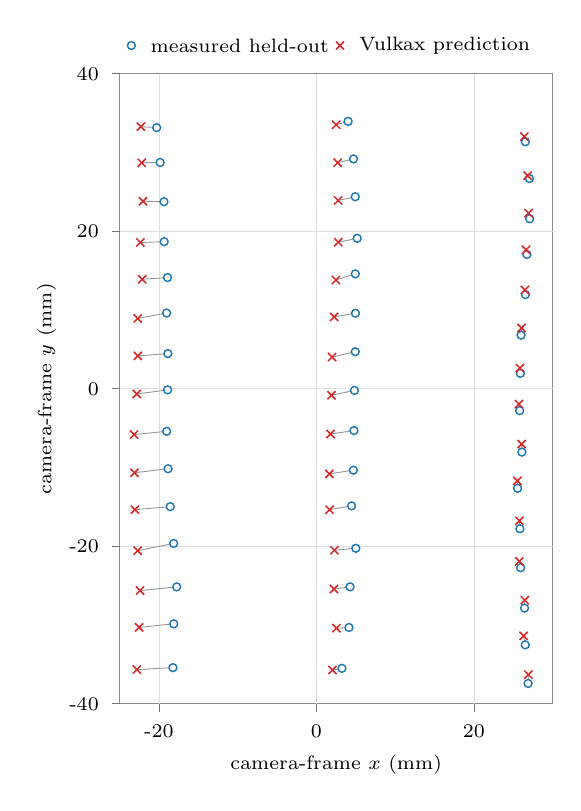
\begin{tikzpicture}[x=1cm,y=1cm]
  \definecolor{dotmeasured}{RGB}{31,119,180}
  \definecolor{dotpredicted}{RGB}{214,39,40}
  \draw[black!45,line width=0.35pt] (0,0) rectangle (5.500,8.000);
  \draw[black!12,line width=0.25pt] (0.500,0) -- (0.500,8.000);
  \draw[black!55,line width=0.3pt] (0.500,0) -- (0.500,-0.10);
  \node[font=\scriptsize,anchor=north] at (0.500,-0.14) {-20};
  \draw[black!12,line width=0.25pt] (2.500,0) -- (2.500,8.000);
  \draw[black!55,line width=0.3pt] (2.500,0) -- (2.500,-0.10);
  \node[font=\scriptsize,anchor=north] at (2.500,-0.14) {0};
  \draw[black!12,line width=0.25pt] (4.500,0) -- (4.500,8.000);
  \draw[black!55,line width=0.3pt] (4.500,0) -- (4.500,-0.10);
  \node[font=\scriptsize,anchor=north] at (4.500,-0.14) {20};
  \draw[black!55,line width=0.3pt] (0,0.000) -- (-0.10,0.000);
  \node[font=\scriptsize,anchor=east] at (-0.14,0.000) {-40};
  \draw[black!12,line width=0.25pt] (0,2.000) -- (5.500,2.000);
  \draw[black!55,line width=0.3pt] (0,2.000) -- (-0.10,2.000);
  \node[font=\scriptsize,anchor=east] at (-0.14,2.000) {-20};
  \draw[black!12,line width=0.25pt] (0,4.000) -- (5.500,4.000);
  \draw[black!55,line width=0.3pt] (0,4.000) -- (-0.10,4.000);
  \node[font=\scriptsize,anchor=east] at (-0.14,4.000) {0};
  \draw[black!12,line width=0.25pt] (0,6.000) -- (5.500,6.000);
  \draw[black!55,line width=0.3pt] (0,6.000) -- (-0.10,6.000);
  \node[font=\scriptsize,anchor=east] at (-0.14,6.000) {20};
  \draw[black!55,line width=0.3pt] (0,8.000) -- (-0.10,8.000);
  \node[font=\scriptsize,anchor=east] at (-0.14,8.000) {40};
  \node[font=\scriptsize,anchor=north] at (2.750,-0.52) {camera-frame $x$ (mm)};
  \node[font=\scriptsize,rotate=90,anchor=south] at (-0.68,4.000) {camera-frame $y$ (mm)};
  \draw[black!42,line width=0.32pt] (0.6777,0.4588) -- (0.2189,0.4347);
  \draw[black!42,line width=0.32pt] (2.8242,0.4503) -- (2.7033,0.4289);
  \draw[black!42,line width=0.32pt] (5.1880,0.2578) -- (5.1911,0.3689);
  \draw[black!42,line width=0.32pt] (0.6878,1.0153) -- (0.2478,0.9708);
  \draw[black!42,line width=0.32pt] (2.9132,0.9690) -- (2.7539,0.9595);
  \draw[black!42,line width=0.32pt] (5.1518,0.7486) -- (5.1308,0.8628);
  \draw[black!42,line width=0.32pt] (0.7254,1.4843) -- (0.2605,1.4379);
  \draw[black!42,line width=0.32pt] (2.9269,1.4853) -- (2.7225,1.4575);
  \draw[black!42,line width=0.32pt] (5.1429,1.2153) -- (5.1458,1.3157);
  \draw[black!42,line width=0.32pt] (0.6868,2.0363) -- (0.2302,1.9444);
  \draw[black!42,line width=0.32pt] (3.0001,1.9747) -- (2.7277,1.9494);
  \draw[black!42,line width=0.32pt] (5.0940,1.7273) -- (5.0761,1.8087);
  \draw[black!42,line width=0.32pt] (0.6438,2.5029) -- (0.1942,2.4662);
  \draw[black!42,line width=0.32pt] (2.9460,2.5137) -- (2.6661,2.4649);
  \draw[black!42,line width=0.32pt] (5.0836,2.2231) -- (5.0779,2.3239);
  \draw[black!42,line width=0.32pt] (0.6158,2.9848) -- (0.1899,2.9342);
  \draw[black!42,line width=0.32pt] (2.9693,2.9665) -- (2.6642,2.9202);
  \draw[black!42,line width=0.32pt] (5.0544,2.7367) -- (5.0519,2.8304);
  \draw[black!42,line width=0.32pt] (0.5979,3.4598) -- (0.1842,3.4188);
  \draw[black!42,line width=0.32pt] (2.9764,3.4694) -- (2.6785,3.4258);
  \draw[black!42,line width=0.32pt] (5.1087,3.1961) -- (5.1057,3.2981);
  \draw[black!42,line width=0.32pt] (0.6100,3.9865) -- (0.2180,3.9343);
  \draw[black!42,line width=0.32pt] (2.9825,3.9794) -- (2.6919,3.9180);
  \draw[black!42,line width=0.32pt] (5.0813,3.7226) -- (5.0720,3.8062);
  \draw[black!42,line width=0.32pt] (0.6130,4.4469) -- (0.2327,4.4185);
  \draw[black!42,line width=0.32pt] (2.9928,4.4712) -- (2.6986,4.4034);
  \draw[black!42,line width=0.32pt] (5.0895,4.1969) -- (5.0840,4.2633);
  \draw[black!42,line width=0.32pt] (0.5973,4.9625) -- (0.2297,4.8933);
  \draw[black!42,line width=0.32pt] (2.9957,4.9600) -- (2.7246,4.9131);
  \draw[black!42,line width=0.32pt] (5.0986,4.6811) -- (5.1046,4.7728);
  \draw[black!42,line width=0.32pt] (0.6087,5.4129) -- (0.2868,5.3913);
  \draw[black!42,line width=0.32pt] (2.9936,5.4597) -- (2.7468,5.3819);
  \draw[black!42,line width=0.32pt] (5.1545,5.1964) -- (5.1486,5.2558);
  \draw[black!42,line width=0.32pt] (0.5664,5.8686) -- (0.2644,5.8581);
  \draw[black!42,line width=0.32pt] (3.0178,5.9113) -- (2.7778,5.8617);
  \draw[black!42,line width=0.32pt] (5.1725,5.7061) -- (5.1628,5.7654);
  \draw[black!42,line width=0.32pt] (0.5635,6.3761) -- (0.2975,6.3826);
  \draw[black!42,line width=0.32pt] (2.9927,6.4391) -- (2.7753,6.3919);
  \draw[black!42,line width=0.32pt] (5.2070,6.1600) -- (5.1931,6.2315);
  \draw[black!42,line width=0.32pt] (0.5147,6.8749) -- (0.2806,6.8707);
  \draw[black!42,line width=0.32pt] (2.9707,6.9204) -- (2.7698,6.8712);
  \draw[black!42,line width=0.32pt] (5.2049,6.6709) -- (5.1822,6.7074);
  \draw[black!42,line width=0.32pt] (0.4711,7.3174) -- (0.2703,7.3292);
  \draw[black!42,line width=0.32pt] (2.9025,7.3963) -- (2.7499,7.3533);
  \draw[black!42,line width=0.32pt] (5.1530,7.1382) -- (5.1404,7.2038);
  \draw[dotmeasured,line width=0.52pt,fill=white] (0.6777,0.4588) circle[radius=0.050];
  \draw[dotmeasured,line width=0.52pt,fill=white] (2.8242,0.4503) circle[radius=0.050];
  \draw[dotmeasured,line width=0.52pt,fill=white] (5.1880,0.2578) circle[radius=0.050];
  \draw[dotmeasured,line width=0.52pt,fill=white] (0.6878,1.0153) circle[radius=0.050];
  \draw[dotmeasured,line width=0.52pt,fill=white] (2.9132,0.9690) circle[radius=0.050];
  \draw[dotmeasured,line width=0.52pt,fill=white] (5.1518,0.7486) circle[radius=0.050];
  \draw[dotmeasured,line width=0.52pt,fill=white] (0.7254,1.4843) circle[radius=0.050];
  \draw[dotmeasured,line width=0.52pt,fill=white] (2.9269,1.4853) circle[radius=0.050];
  \draw[dotmeasured,line width=0.52pt,fill=white] (5.1429,1.2153) circle[radius=0.050];
  \draw[dotmeasured,line width=0.52pt,fill=white] (0.6868,2.0363) circle[radius=0.050];
  \draw[dotmeasured,line width=0.52pt,fill=white] (3.0001,1.9747) circle[radius=0.050];
  \draw[dotmeasured,line width=0.52pt,fill=white] (5.0940,1.7273) circle[radius=0.050];
  \draw[dotmeasured,line width=0.52pt,fill=white] (0.6438,2.5029) circle[radius=0.050];
  \draw[dotmeasured,line width=0.52pt,fill=white] (2.9460,2.5137) circle[radius=0.050];
  \draw[dotmeasured,line width=0.52pt,fill=white] (5.0836,2.2231) circle[radius=0.050];
  \draw[dotmeasured,line width=0.52pt,fill=white] (0.6158,2.9848) circle[radius=0.050];
  \draw[dotmeasured,line width=0.52pt,fill=white] (2.9693,2.9665) circle[radius=0.050];
  \draw[dotmeasured,line width=0.52pt,fill=white] (5.0544,2.7367) circle[radius=0.050];
  \draw[dotmeasured,line width=0.52pt,fill=white] (0.5979,3.4598) circle[radius=0.050];
  \draw[dotmeasured,line width=0.52pt,fill=white] (2.9764,3.4694) circle[radius=0.050];
  \draw[dotmeasured,line width=0.52pt,fill=white] (5.1087,3.1961) circle[radius=0.050];
  \draw[dotmeasured,line width=0.52pt,fill=white] (0.6100,3.9865) circle[radius=0.050];
  \draw[dotmeasured,line width=0.52pt,fill=white] (2.9825,3.9794) circle[radius=0.050];
  \draw[dotmeasured,line width=0.52pt,fill=white] (5.0813,3.7226) circle[radius=0.050];
  \draw[dotmeasured,line width=0.52pt,fill=white] (0.6130,4.4469) circle[radius=0.050];
  \draw[dotmeasured,line width=0.52pt,fill=white] (2.9928,4.4712) circle[radius=0.050];
  \draw[dotmeasured,line width=0.52pt,fill=white] (5.0895,4.1969) circle[radius=0.050];
  \draw[dotmeasured,line width=0.52pt,fill=white] (0.5973,4.9625) circle[radius=0.050];
  \draw[dotmeasured,line width=0.52pt,fill=white] (2.9957,4.9600) circle[radius=0.050];
  \draw[dotmeasured,line width=0.52pt,fill=white] (5.0986,4.6811) circle[radius=0.050];
  \draw[dotmeasured,line width=0.52pt,fill=white] (0.6087,5.4129) circle[radius=0.050];
  \draw[dotmeasured,line width=0.52pt,fill=white] (2.9936,5.4597) circle[radius=0.050];
  \draw[dotmeasured,line width=0.52pt,fill=white] (5.1545,5.1964) circle[radius=0.050];
  \draw[dotmeasured,line width=0.52pt,fill=white] (0.5664,5.8686) circle[radius=0.050];
  \draw[dotmeasured,line width=0.52pt,fill=white] (3.0178,5.9113) circle[radius=0.050];
  \draw[dotmeasured,line width=0.52pt,fill=white] (5.1725,5.7061) circle[radius=0.050];
  \draw[dotmeasured,line width=0.52pt,fill=white] (0.5635,6.3761) circle[radius=0.050];
  \draw[dotmeasured,line width=0.52pt,fill=white] (2.9927,6.4391) circle[radius=0.050];
  \draw[dotmeasured,line width=0.52pt,fill=white] (5.2070,6.1600) circle[radius=0.050];
  \draw[dotmeasured,line width=0.52pt,fill=white] (0.5147,6.8749) circle[radius=0.050];
  \draw[dotmeasured,line width=0.52pt,fill=white] (2.9707,6.9204) circle[radius=0.050];
  \draw[dotmeasured,line width=0.52pt,fill=white] (5.2049,6.6709) circle[radius=0.050];
  \draw[dotmeasured,line width=0.52pt,fill=white] (0.4711,7.3174) circle[radius=0.050];
  \draw[dotmeasured,line width=0.52pt,fill=white] (2.9025,7.3963) circle[radius=0.050];
  \draw[dotmeasured,line width=0.52pt,fill=white] (5.1530,7.1382) circle[radius=0.050];
  \draw[dotpredicted,line width=0.55pt] (0.1669,0.3827) -- (0.2709,0.4867);
  \draw[dotpredicted,line width=0.55pt] (0.1669,0.4867) -- (0.2709,0.3827);
  \draw[dotpredicted,line width=0.55pt] (2.6513,0.3769) -- (2.7553,0.4809);
  \draw[dotpredicted,line width=0.55pt] (2.6513,0.4809) -- (2.7553,0.3769);
  \draw[dotpredicted,line width=0.55pt] (5.1391,0.3169) -- (5.2431,0.4209);
  \draw[dotpredicted,line width=0.55pt] (5.1391,0.4209) -- (5.2431,0.3169);
  \draw[dotpredicted,line width=0.55pt] (0.1958,0.9188) -- (0.2998,1.0228);
  \draw[dotpredicted,line width=0.55pt] (0.1958,1.0228) -- (0.2998,0.9188);
  \draw[dotpredicted,line width=0.55pt] (2.7019,0.9075) -- (2.8059,1.0115);
  \draw[dotpredicted,line width=0.55pt] (2.7019,1.0115) -- (2.8059,0.9075);
  \draw[dotpredicted,line width=0.55pt] (5.0788,0.8108) -- (5.1828,0.9148);
  \draw[dotpredicted,line width=0.55pt] (5.0788,0.9148) -- (5.1828,0.8108);
  \draw[dotpredicted,line width=0.55pt] (0.2085,1.3859) -- (0.3125,1.4899);
  \draw[dotpredicted,line width=0.55pt] (0.2085,1.4899) -- (0.3125,1.3859);
  \draw[dotpredicted,line width=0.55pt] (2.6705,1.4055) -- (2.7745,1.5095);
  \draw[dotpredicted,line width=0.55pt] (2.6705,1.5095) -- (2.7745,1.4055);
  \draw[dotpredicted,line width=0.55pt] (5.0938,1.2637) -- (5.1978,1.3677);
  \draw[dotpredicted,line width=0.55pt] (5.0938,1.3677) -- (5.1978,1.2637);
  \draw[dotpredicted,line width=0.55pt] (0.1782,1.8924) -- (0.2822,1.9964);
  \draw[dotpredicted,line width=0.55pt] (0.1782,1.9964) -- (0.2822,1.8924);
  \draw[dotpredicted,line width=0.55pt] (2.6757,1.8974) -- (2.7797,2.0014);
  \draw[dotpredicted,line width=0.55pt] (2.6757,2.0014) -- (2.7797,1.8974);
  \draw[dotpredicted,line width=0.55pt] (5.0241,1.7567) -- (5.1281,1.8607);
  \draw[dotpredicted,line width=0.55pt] (5.0241,1.8607) -- (5.1281,1.7567);
  \draw[dotpredicted,line width=0.55pt] (0.1422,2.4142) -- (0.2462,2.5182);
  \draw[dotpredicted,line width=0.55pt] (0.1422,2.5182) -- (0.2462,2.4142);
  \draw[dotpredicted,line width=0.55pt] (2.6141,2.4129) -- (2.7181,2.5169);
  \draw[dotpredicted,line width=0.55pt] (2.6141,2.5169) -- (2.7181,2.4129);
  \draw[dotpredicted,line width=0.55pt] (5.0259,2.2719) -- (5.1299,2.3759);
  \draw[dotpredicted,line width=0.55pt] (5.0259,2.3759) -- (5.1299,2.2719);
  \draw[dotpredicted,line width=0.55pt] (0.1379,2.8822) -- (0.2419,2.9862);
  \draw[dotpredicted,line width=0.55pt] (0.1379,2.9862) -- (0.2419,2.8822);
  \draw[dotpredicted,line width=0.55pt] (2.6122,2.8682) -- (2.7162,2.9722);
  \draw[dotpredicted,line width=0.55pt] (2.6122,2.9722) -- (2.7162,2.8682);
  \draw[dotpredicted,line width=0.55pt] (4.9999,2.7784) -- (5.1039,2.8824);
  \draw[dotpredicted,line width=0.55pt] (4.9999,2.8824) -- (5.1039,2.7784);
  \draw[dotpredicted,line width=0.55pt] (0.1322,3.3668) -- (0.2362,3.4708);
  \draw[dotpredicted,line width=0.55pt] (0.1322,3.4708) -- (0.2362,3.3668);
  \draw[dotpredicted,line width=0.55pt] (2.6265,3.3738) -- (2.7305,3.4778);
  \draw[dotpredicted,line width=0.55pt] (2.6265,3.4778) -- (2.7305,3.3738);
  \draw[dotpredicted,line width=0.55pt] (5.0537,3.2461) -- (5.1577,3.3501);
  \draw[dotpredicted,line width=0.55pt] (5.0537,3.3501) -- (5.1577,3.2461);
  \draw[dotpredicted,line width=0.55pt] (0.1660,3.8823) -- (0.2700,3.9863);
  \draw[dotpredicted,line width=0.55pt] (0.1660,3.9863) -- (0.2700,3.8823);
  \draw[dotpredicted,line width=0.55pt] (2.6399,3.8660) -- (2.7439,3.9700);
  \draw[dotpredicted,line width=0.55pt] (2.6399,3.9700) -- (2.7439,3.8660);
  \draw[dotpredicted,line width=0.55pt] (5.0200,3.7542) -- (5.1240,3.8582);
  \draw[dotpredicted,line width=0.55pt] (5.0200,3.8582) -- (5.1240,3.7542);
  \draw[dotpredicted,line width=0.55pt] (0.1807,4.3665) -- (0.2847,4.4705);
  \draw[dotpredicted,line width=0.55pt] (0.1807,4.4705) -- (0.2847,4.3665);
  \draw[dotpredicted,line width=0.55pt] (2.6466,4.3514) -- (2.7506,4.4554);
  \draw[dotpredicted,line width=0.55pt] (2.6466,4.4554) -- (2.7506,4.3514);
  \draw[dotpredicted,line width=0.55pt] (5.0320,4.2113) -- (5.1360,4.3153);
  \draw[dotpredicted,line width=0.55pt] (5.0320,4.3153) -- (5.1360,4.2113);
  \draw[dotpredicted,line width=0.55pt] (0.1777,4.8413) -- (0.2817,4.9453);
  \draw[dotpredicted,line width=0.55pt] (0.1777,4.9453) -- (0.2817,4.8413);
  \draw[dotpredicted,line width=0.55pt] (2.6726,4.8611) -- (2.7766,4.9651);
  \draw[dotpredicted,line width=0.55pt] (2.6726,4.9651) -- (2.7766,4.8611);
  \draw[dotpredicted,line width=0.55pt] (5.0526,4.7208) -- (5.1566,4.8248);
  \draw[dotpredicted,line width=0.55pt] (5.0526,4.8248) -- (5.1566,4.7208);
  \draw[dotpredicted,line width=0.55pt] (0.2348,5.3393) -- (0.3388,5.4433);
  \draw[dotpredicted,line width=0.55pt] (0.2348,5.4433) -- (0.3388,5.3393);
  \draw[dotpredicted,line width=0.55pt] (2.6948,5.3299) -- (2.7988,5.4339);
  \draw[dotpredicted,line width=0.55pt] (2.6948,5.4339) -- (2.7988,5.3299);
  \draw[dotpredicted,line width=0.55pt] (5.0966,5.2038) -- (5.2006,5.3078);
  \draw[dotpredicted,line width=0.55pt] (5.0966,5.3078) -- (5.2006,5.2038);
  \draw[dotpredicted,line width=0.55pt] (0.2124,5.8061) -- (0.3164,5.9101);
  \draw[dotpredicted,line width=0.55pt] (0.2124,5.9101) -- (0.3164,5.8061);
  \draw[dotpredicted,line width=0.55pt] (2.7258,5.8097) -- (2.8298,5.9137);
  \draw[dotpredicted,line width=0.55pt] (2.7258,5.9137) -- (2.8298,5.8097);
  \draw[dotpredicted,line width=0.55pt] (5.1108,5.7134) -- (5.2148,5.8174);
  \draw[dotpredicted,line width=0.55pt] (5.1108,5.8174) -- (5.2148,5.7134);
  \draw[dotpredicted,line width=0.55pt] (0.2455,6.3306) -- (0.3495,6.4346);
  \draw[dotpredicted,line width=0.55pt] (0.2455,6.4346) -- (0.3495,6.3306);
  \draw[dotpredicted,line width=0.55pt] (2.7233,6.3399) -- (2.8273,6.4439);
  \draw[dotpredicted,line width=0.55pt] (2.7233,6.4439) -- (2.8273,6.3399);
  \draw[dotpredicted,line width=0.55pt] (5.1411,6.1795) -- (5.2451,6.2835);
  \draw[dotpredicted,line width=0.55pt] (5.1411,6.2835) -- (5.2451,6.1795);
  \draw[dotpredicted,line width=0.55pt] (0.2286,6.8187) -- (0.3326,6.9227);
  \draw[dotpredicted,line width=0.55pt] (0.2286,6.9227) -- (0.3326,6.8187);
  \draw[dotpredicted,line width=0.55pt] (2.7178,6.8192) -- (2.8218,6.9232);
  \draw[dotpredicted,line width=0.55pt] (2.7178,6.9232) -- (2.8218,6.8192);
  \draw[dotpredicted,line width=0.55pt] (5.1302,6.6554) -- (5.2342,6.7594);
  \draw[dotpredicted,line width=0.55pt] (5.1302,6.7594) -- (5.2342,6.6554);
  \draw[dotpredicted,line width=0.55pt] (0.2183,7.2772) -- (0.3223,7.3812);
  \draw[dotpredicted,line width=0.55pt] (0.2183,7.3812) -- (0.3223,7.2772);
  \draw[dotpredicted,line width=0.55pt] (2.6979,7.3013) -- (2.8019,7.4053);
  \draw[dotpredicted,line width=0.55pt] (2.6979,7.4053) -- (2.8019,7.3013);
  \draw[dotpredicted,line width=0.55pt] (5.0884,7.1518) -- (5.1924,7.2558);
  \draw[dotpredicted,line width=0.55pt] (5.0884,7.2558) -- (5.1924,7.1518);
  \draw[dotmeasured,line width=0.52pt,fill=white] (0.15,8.360) circle[radius=0.050];
  \node[font=\scriptsize,anchor=west] at (0.27,8.360) {measured held-out};
  \draw[dotpredicted,line width=0.55pt] (2.75,8.310) -- (2.85,8.410);
  \draw[dotpredicted,line width=0.55pt] (2.75,8.410) -- (2.85,8.310);
  \node[font=\scriptsize,anchor=west] at (2.92,8.360) {Vulkax prediction};
\end{tikzpicture}
}
\caption{Held-out DOT C2 measured-versus-predicted geometry at \(t=0.167\) s in the camera-frame \(x/y\) projection. Circles are measured correspondences, crosses are predictions, and connecting segments are true-scale residuals. Across the 90 held-out samples from both nonzero checkpoints, the 3-D RMS is 4.417 mm.}
\label{fig:dot-c2-heldout}
\end{figure}

GAUGE contributes two distinct measured protocols. GAUGE is retrospective in the foam-shearing analysis, which compares ordinary face/marker error with a longitudinal mechanism channel over ten held-out repeats. The prospective lane is frozen separately on foam stretching and compression, soft and hard materials, and repeats 5--7. That validation partition contains 12 measured worlds and three predeclared cases per world: SUPPORT, VETO, and placebo/UNRESOLVED. Repeats 8--10 are reserved as final media and remain unopened after the validation gate fails.

\subsection{Fresh orthogonal force-compliance protocol}\label{fresh-orthogonal-force-compliance-study}

The force-compliance experiment changes the verification channel while keeping proposal generation fixed. Fresh prospective force evidence is synthetic in this study; no measured force-sensor verification claim is made. It evaluates 36 fresh synthetic proposals, of which 12 are deceptive and 24 beneficial on the untouched target. Fresh DCS and force compliance share the same decision magnitude \(\tau=2\).

The advancement gate is frozen before execution. It requires at least four deceptive repairs, at least 30\% resolved force coverage, at least 50\% veto recall on deceptive repairs, at most 25\% false-veto rate on beneficial repairs, force coverage greater than DCS coverage, a higher force median \(|z|\), and finite numerical comparisons for every proposal. A later threshold sweep is post hoc and cannot redefine this gate.

\begin{figure}
\centering
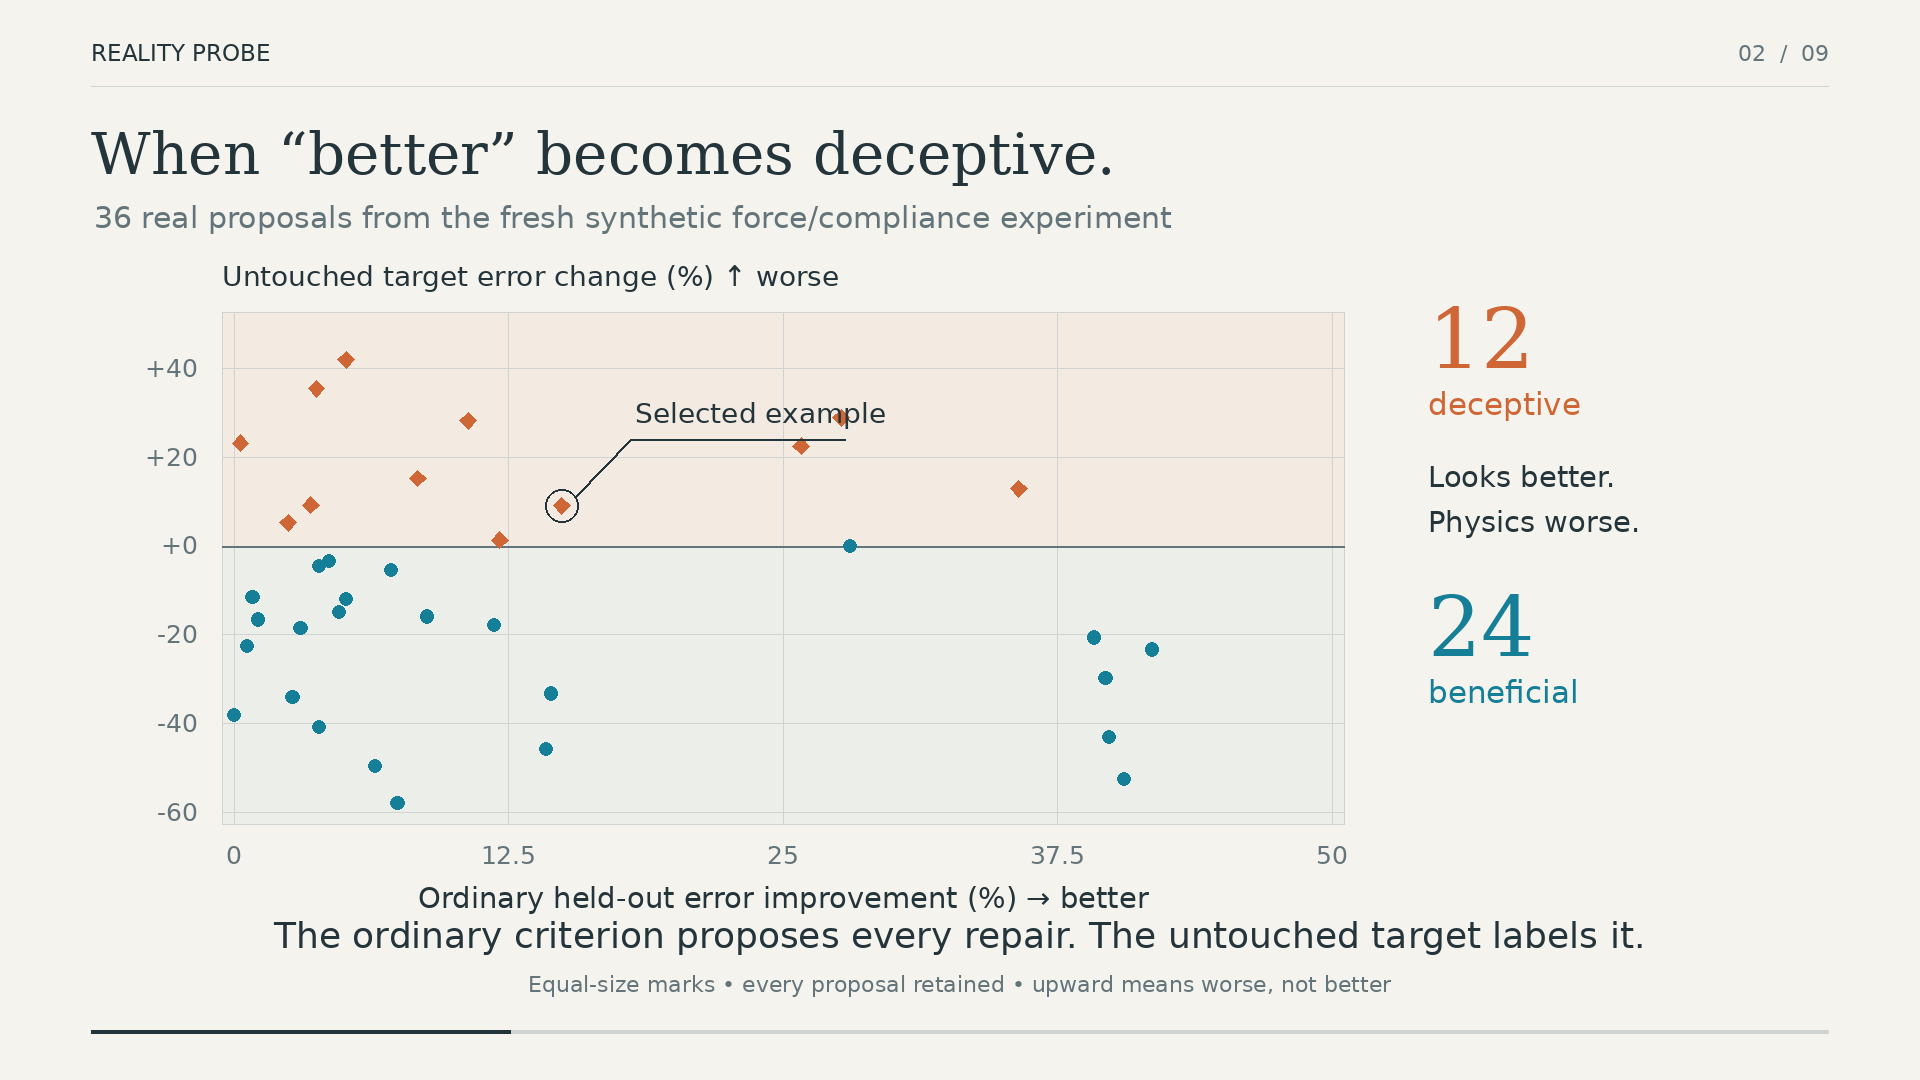
\includegraphics[width=\linewidth]{../docs/readme_assets/03_deception_map.png}
\caption{Fresh force-compliance proposal population. Ordinary held-out improvement and untouched-target behavior disagree for part of the population, producing both deceptive and beneficial rewrites.}
\label{fig:deception-map}
\end{figure}

\subsection{Locked IRIS pendulum protocol and post-final analyses}\label{locked-iris-pendulum-protocol}

The measured positive test uses IRIS \texttt{pendulum\_90}. The tracker, candidate schedule, decision magnitude, and final media are repository-frozen before the 10-video final set is opened. The primary verifier uses the finite-amplitude pendulum period relation. The matched diagnostic baseline uses the small-angle approximation. Each physical video generates 11 controlled SUPPORT/VETO/UNRESOLVED cases, for 110 nested case rows across 10 videos.

Post-final analyses form a separate evidence class. They resample at the physical-video level, compare two additional pendulum residual models, generate GT-hidden proposals from early video segments, vary proposal/probe overlap, propagate recorded rope-length uncertainty, and stress the locked decision under image corruption and temporal downsampling. None of these analyses can replace or retune the locked final result.

\subsection{Frozen IRIS free-fall transfer test}\label{frozen-iris-free-fall-protocol}

The free-fall lane tests a different equation family with a separately frozen protocol. Development uses \texttt{drop\_50/06..10}; validation uses untouched \texttt{drop\_100/06..10}; the designated final set is \texttt{drop\_150/02..10}. The V6.6 policy forbids threshold retuning, tracker changes, candidate changes, or scene substitution after lock. Validation is opened only after the development gate passes. A failed validation permanently removes that split from confirmatory use and prevents the final set from being opened.

\section{Results and Analysis}\label{results-and-analysis}

\subsection{Ordinary improvement can hide physical degradation}\label{deceptive-repair-is-a-distinct-failure-mode}

The deceptive-repair condition appears in both controlled ordinary-improving populations. D4V contains 14 deceptive repairs among 36 proposals; the fresh force-compliance population contains 12 among 36. These fractions describe the constructed candidate populations and should not be interpreted as a universal deception rate. Their role is narrower: an approval rule based only on ordinary held-out improvement would accept candidates that are worse on an untouched physical target.

Figure~\ref{fig:deceptive-repair} shows one such case. The candidate lowers ordinary held-out error by 14.93\% while increasing untouched-target error by 9.03\%. The measured observation is the disagreement between those two evaluation channels. The interpretation is that ordinary held-out fit alone is insufficient for deciding whether this physical rewrite should be committed.

\subsection{DCS succeeds in the control and remains information-poor prospectively}\label{the-dcs-hypothesis-is-falsified-as-a-general-prospective-verifier}

D1 confirms that the implementation can express a strong dark-field rejection: all 64 constructed deceptive repairs improve the ordinary criterion and all 64 are rejected by DCS. Median ordinary improvement is 60.88\%, and the median witness-degradation ratio is 9.375.

The prospective stages are much weaker. In D2 discovery, ranking agreement is 95.83\% for raw maximin, 87.50\% for Fisher/Jacobian selection, 75.00\% for the same-cost raw bundle, 66.67\% for maximum motion, 62.50\% for DCS order-2 maximin, and 45.83\% for random selection. DCS is therefore not the strongest matched ranking method in that comparison. On the 16 frozen D2 truth worlds, no witness reaches the decision magnitude; median standardized separation is 0.041578. Median numerical RMS is \(6.469\times10^{-6}\) m and the maximum moment residual is \(3.886\times10^{-16}\). The cancellation algebra is numerically well behaved while the physical alternatives remain weakly separated.

D3 tests whether solver refinement recovers the missing separation. Adaptive selection chooses order 2 on all six fresh worlds, and the median standardized separation is 0.0588583. Refinement lowers median numerical RMS from \(8.435\times10^{-7}\) m for order 2 to \(2.153\times10^{-7}\) m for order 3, yet no world is resolved. Ranking agreement remains modest: Fisher 61.11\%, raw bundle 58.33\%, maximum motion 58.33\%, pair-aware raw 55.56\%, adaptive DCS 52.78\%, and order-3 DCS 47.22\%.

This separates numerical accuracy from physical observability. The refined witness is numerically cleaner, but the evidence available to distinguish the candidate worlds barely changes.

D4V reaches the same decision-level outcome on ordinary-improving proposals. DCS, raw bundle, pair-specific raw, Fisher, and maximum-motion verification all have 0/36 resolved coverage at \(|z|\ge2\). The post-hoc information-frontier calculation quantifies the remaining gap: median DCS magnitude is 0.05024, corresponding to roughly 39.8\(\times\) median amplification to reach magnitude 2 if the uncertainty scale were unchanged. This number is a diagnostic of missing evidence, not a revised threshold.

\subsection{Measured GAUGE channels disagree and remain below the frozen decision scale}\label{measured-gauge-results}

The retrospective GAUGE shearing analysis shows a measured channel contradiction. Ordinary face-plus-marker metrics prefer the finite-overlap candidate in all ten repeats, and marker dark-field agrees. The longitudinal mechanism channel prefers the endpoint model in 9/10 repeats. Median marker error is 0.002428 m for endpoint and 0.001709 m for overlap, whereas median longitudinal error is 0.003131 for endpoint and 0.005584 for overlap. A post-hoc exact two-sided sign test on the longitudinal direction gives \(p=0.02148\).

\begin{table}[t]
\centering
\caption{Retrospective GAUGE shearing comparison. Lower error is better. The sign test is post hoc.}
\label{tab:gauge}
\begin{tabular}{lcc}
\toprule
Metric & Endpoint & Overlap \\
\midrule
Median marker error (m) & 0.002428 & 0.001709 \\
Median longitudinal error & 0.003131 & 0.005584 \\
Longitudinal held-out wins & 9/10 & 1/10 \\
\bottomrule
\end{tabular}
\end{table}

The separately frozen GAUGE validation lane provides a prospective measured failure. Across 12 stretching/compression worlds, the temporal annihilating witness makes 0/12 correct SUPPORT decisions and 0/12 correct VETO decisions, while all 12 placebo cases remain UNRESOLVED. Saved-output forensics show correct raw truth ordering on every directional case. The median raw signal is only 0.00277 times the repeat variability and 0.1179 times the nominal-versus-refined numerical discrepancy. The evidence therefore points to an information-limited channel under the frozen probe rather than a reversal of the underlying truth ordering. Repeats 8--10 remain unopened.

\subsection{Known-force compliance changes the evidence scale but does not clear the gate}\label{orthogonal-physical-information-changes-the-evidence-scale}

Fresh DCS on the orthogonal-information population has median \(|z|=0.04877\) and maximum \(|z|=0.17279\). Known-force compliance raises the median to 0.55863 and the maximum to 1.31911. The aggregate median-magnitude ratio is 11.455\(\times\).

\begin{table}[t]
\centering
\caption{Fresh synthetic force-compliance results under the common frozen decision magnitude.}
\label{tab:ofc}
\begin{tabular}{lcc}
\toprule
Quantity & DCS & Force compliance \\
\midrule
Median \(|z|\) & 0.04877 & 0.55863 \\
Maximum \(|z|\) & 0.17279 & 1.31911 \\
Resolved coverage & 0/36 & 0/36 \\
Median factor to \(|z|=2\) & 41.01\(\times\) & 3.58\(\times\) \\
Best-case factor to \(|z|=2\) & 11.57\(\times\) & 1.52\(\times\) \\
\bottomrule
\end{tabular}
\end{table}

\begin{figure}
\centering
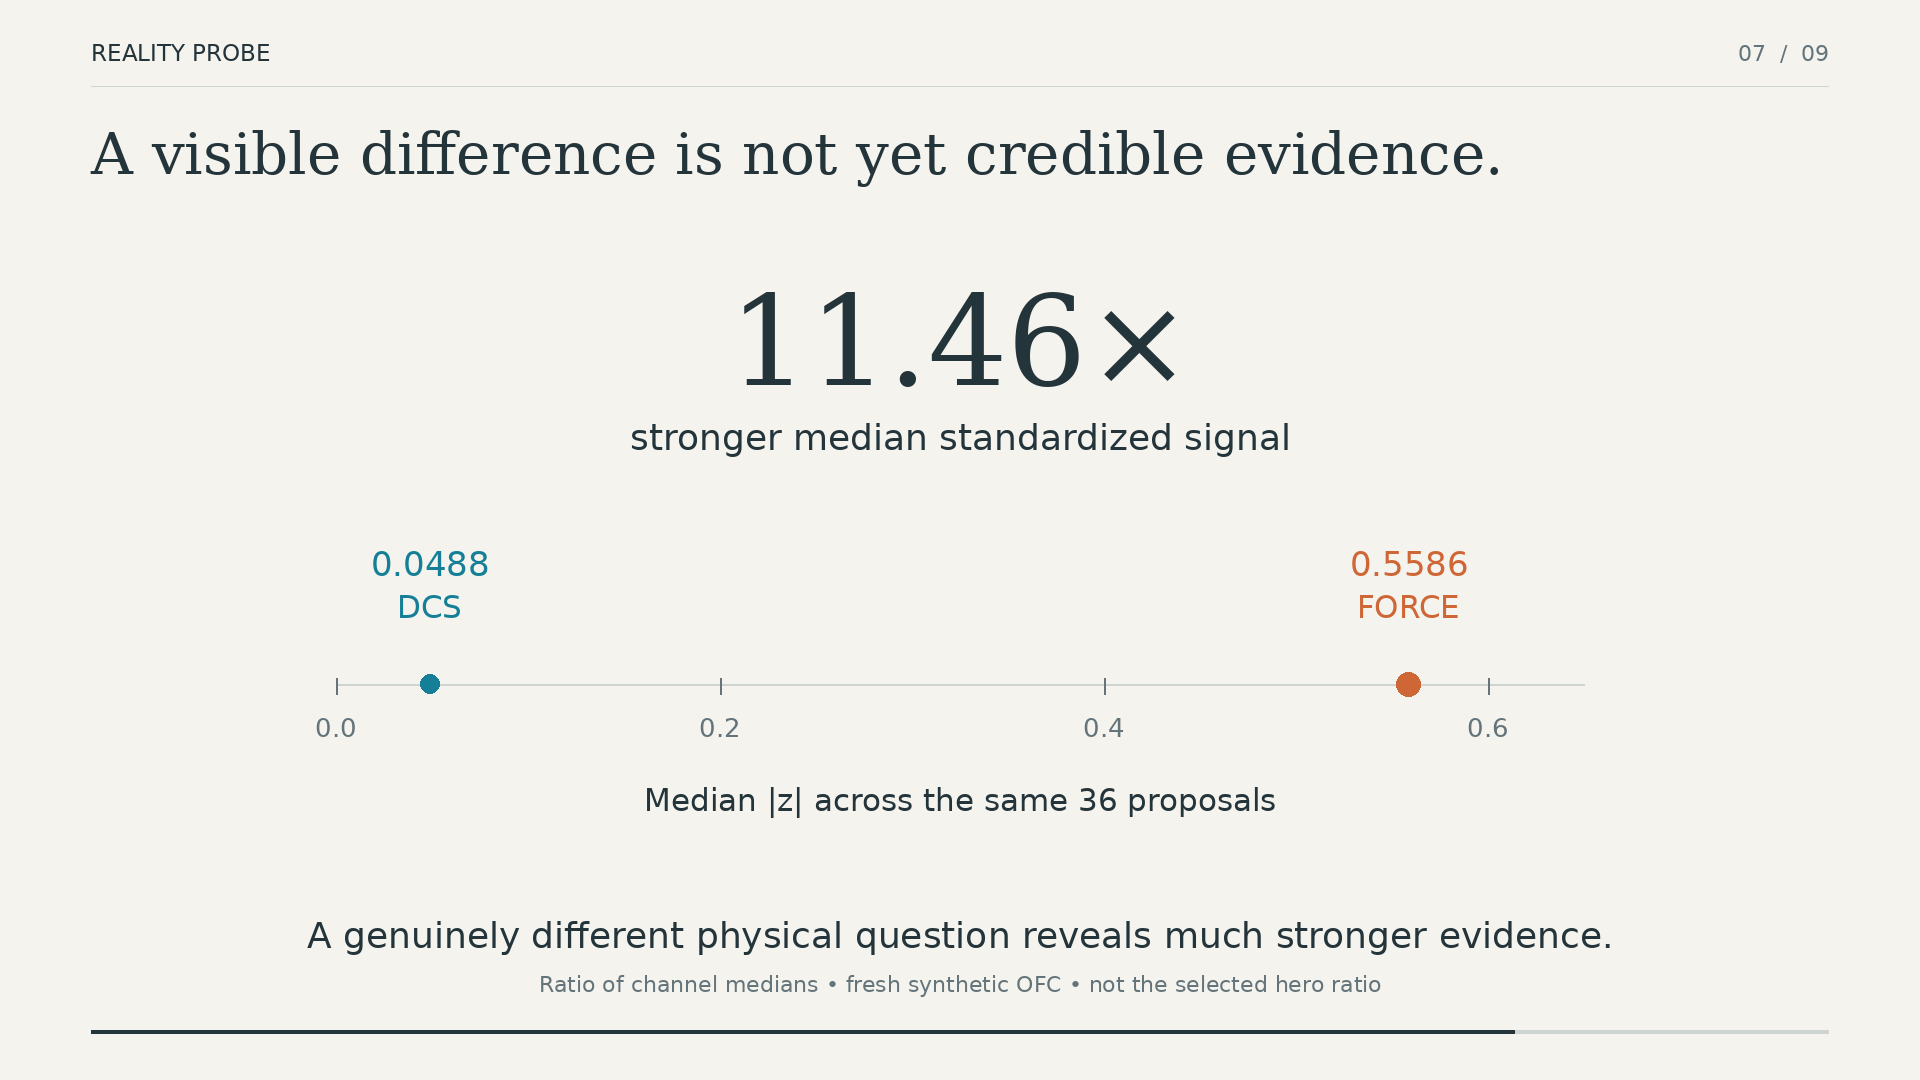
\includegraphics[width=\linewidth]{../docs/readme_assets/10_signal_gain.png}
\caption{Fresh known-force compliance raises median standardized evidence magnitude by 11.46\(\times\) relative to fresh DCS under the same decision rule.}
\label{fig:signal-gain}
\end{figure}

The evidence scale changes substantially, but the frozen advancement gate still fails. Force compliance resolves 0/36 proposals, so resolved coverage and deceptive-repair veto recall do not meet their required minima. The population-size, beneficial false-veto, median-signal, and numerical-comparison conditions pass. The observation is therefore precise: this physical channel carries more discriminating information than fresh DCS, but the measured separation remains insufficient for a SUPPORT/VETO decision at \(\tau=2\).

A post-hoc threshold sweep checks how quickly that conclusion changes as the decision magnitude is relaxed. Fresh DCS has no crossing even at \(\tau=1\). Force compliance resolves 14/36 proposals at \(\tau=1\): six SUPPORT and eight VETO. Five of the 12 deceptive repairs are vetoed, giving 41.7\% recall, and three of the 24 beneficial repairs are falsely vetoed, giving 12.5\% false-veto rate. At \(\tau=1.5\) and above, coverage returns to 0/36. The sweep describes the score distribution; it does not redefine the prospectively frozen policy.

\begin{table}[t]
\centering
\caption{Post-hoc threshold sensitivity from the frozen per-proposal ledger. The \(\tau=2\) row is the repository-frozen primary rule.}
\label{tab:threshold-sensitivity}
\begin{tabular}{lcc}
\toprule
Decision magnitude \(\tau\) & DCS crossings & Force crossings \\
\midrule
1.0 & 0/36 & 14/36 \\
1.5 & 0/36 & 0/36 \\
2.0 & 0/36 & 0/36 \\
2.5 & 0/36 & 0/36 \\
3.0 & 0/36 & 0/36 \\
\bottomrule
\end{tabular}
\end{table}

\begin{figure}
\centering
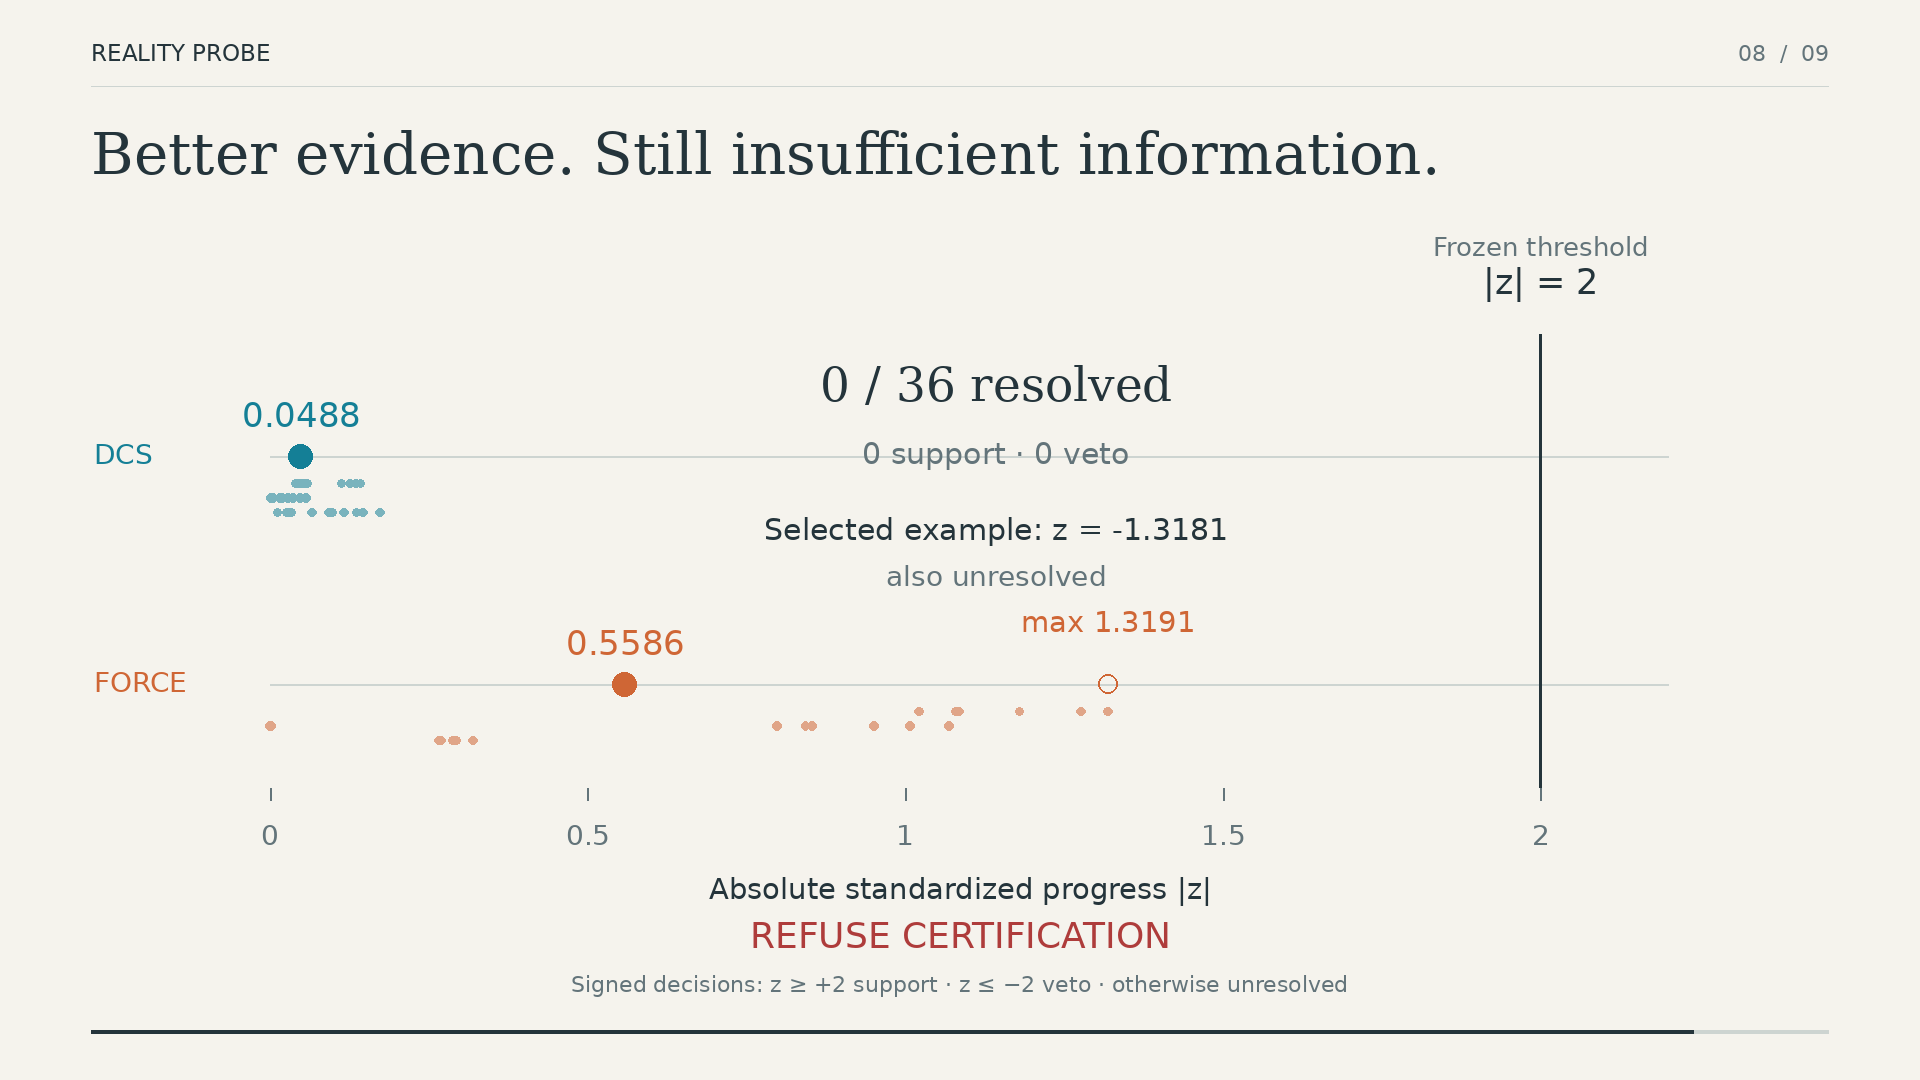
\includegraphics[width=\linewidth]{../docs/readme_assets/11_information_limit.png}
\caption{Information-frontier view of the fresh synthetic experiment. Force compliance moves the evidence closer to the frozen decision magnitude, but even the strongest proposal remains below it.}
\label{fig:information-limit}
\end{figure}

\subsection{The locked pendulum test provides a measured positive case}\label{locked-iris-pendulum-confirmation}

All ten final \texttt{pendulum\_90} videos pass the quality gate. Across the 110 controlled cases nested within those videos, the finite-amplitude probe makes 90 decisions correctly (81.82\%). The small-angle diagnostic baseline makes 40/110 correctly (36.36\%). The primary probe is correct on 40/50 SUPPORT cases, 40/50 VETO cases, and all 10 UNRESOLVED placebo cases. In the paired case table, the primary probe is correct when the baseline is not on 50 cases; the reverse occurs on zero cases, with 60 ties. The locked physical-recovery diagnostic has 16.81\% median relative error in period-inferred pendulum length.

The physical video is the correct inference unit. A post-final clustered analysis therefore resamples the ten videos rather than the 110 nested rows. Per-video strict accuracies are identical across the ten final videos, giving primary accuracy 0.8182, baseline accuracy 0.3636, and a difference of 0.4545 in every video-level bootstrap resample. More directly, the primary probe beats the baseline on 10/10 videos with no ties; the exact two-sided sign-test value is \(p=0.001953125\).

Two additional post-final residual comparators do not explain away the locked result. A direct finite-amplitude period residual reaches 45.45\% strict three-way accuracy, and a damped nonlinear ODE residual reaches 9.09\%; both retain 100\% placebo accuracy. Relative to the direct residual, the locked primary is uniquely correct on 40 cases and the comparator on zero. Relative to the damped ODE residual, the corresponding counts are 80 and zero. These are secondary comparisons and do not replace the locked primary-baseline result.

The GT-hidden post-final proposal test removes the manually scheduled candidate factors. For each video, an early segment generates the proposal and a later segment evaluates ordinary improvement. The blind proposal file is hashed before ground truth is joined. All ten proposals improve the ordinary holdout; eight are physically worse and two are physically better. The reserved final-window verifier classifies all ten correctly. Varying proposal/probe overlap from \(\rho=0\) to \(\rho=1\) leaves these ten post-final decisions correct throughout, with median absolute score decreasing from 18.08 to 16.21. This tests dependence on temporal partition choice; it does not make two windows from the same video independent sensor modalities.

Recorded rope-length uncertainty also leaves the controlled truth labels unchanged: all 110 labels remain stable at both \(\pm1\sigma\) and \(\pm2\sigma\). The full corruption suite runs 180 condition-video combinations with no failed videos. The clean Metal path reproduces the locked decision vector on all ten videos. Tested noise, blur, frame duplication/drop, central occlusion, and crop levels preserve 81.82\% strict accuracy. Temporal downsampling exposes the clear boundary: accuracy falls to 63.64\% at 30 fps and 45.45\% at 15 fps, while placebo accuracy remains 100\%.

The measured observation is therefore specific but useful. A pendulum-specific observable supports accurate SUPPORT/VETO decisions on fresh video under the locked protocol, while the post-final stress tests identify temporal resolution as an acquisition constraint.

\subsection{The free-fall transfer test fails validation}\label{second-domain-iris-free-fall-failure}

V6.6 passes its \texttt{drop\_50} development gate before validation is opened: 4/5 videos pass quality, there are zero implementation errors, and median acceleration relative error is 8.05\%. Take 07 is excluded because no causal release-to-terminal-impact event survives the frozen selector.

The untouched \texttt{drop\_100/06..10} validation split then fails. All five videos pass the low-level quality checks, but median acceleration relative error is 111.7\%. Truth-control accuracy is 0 and direction-sign rate is 0 under the frozen logic. The selected intervals imply approximately 15.0--19.4 frames of full-fall time, whereas a 1 m release-from-rest fall at \(g=9.80665\) m/s\(^2\) is about 27.1 frames at 60 fps.

That discrepancy motivates a post-validation hypothesis: the selector is often finding a locally ballistic partial interval and then assigning the full known 1 m height to it. Retrospective diagnostics support the partial-flight signature but do not produce a valid repair. Global/chunk scaling, stationary endpoint anchors, fragmented-track stitching, 16 resolution/association/ranking variants, and bidirectional hold-to-hold reconstruction all fail to produce a robust target-free estimator across the spent development and validation evidence.

The frozen protocol determines the disposition. \texttt{drop\_100} is permanently retrospective, the rescue analyses remain diagnostic, and \texttt{drop\_150/02..10} stays unopened. This second domain therefore contributes a boundary result, not a second success.

\subsection{The sequence isolates an information problem}\label{stronger-evidence-is-not-sufficient-evidence}

Across the full program, implementation validity, evidence magnitude, and decision sufficiency separate cleanly. DCS can be numerically well behaved while far below the decision scale. A different physical channel can increase standardized evidence by more than an order of magnitude and still remain unresolved. A pendulum-specific observable can cross the decision boundary reliably on fresh measured video. A free-fall estimator that appears adequate in development can fail untouched validation.

The interpretation supported by this sequence is that verification quality depends on the information supplied by the experiment, not only on the estimator applied afterward. Reality Probe makes that dependency visible because weak evidence stays unresolved and failed validation remains failed.

\section{Discussion}\label{discussion}

\subsection{Why the channels behave differently}\label{why-the-channels-behave-differently}

The synthetic sequence rules out a simple implementation explanation for the weak DCS results. D1 shows that the code path can produce strong rejection when the contrast is deliberately present. D2 and D3 show that moment cancellation and numerical refinement can remain well behaved while standardized separation stays far below the decision magnitude. D4V extends that observation to actual ordinary-improving proposals.

Changing the physical question has a larger effect than refining the original witness. Known-force compliance increases median evidence magnitude by 11.46\(\times\) on fresh synthetic worlds. The pendulum experiment goes further: a physical observable tied directly to the governing period relation produces useful decisions on fresh measured video. The free-fall lane then shows the opposite boundary. A locally plausible event detector passes development but fails when the observed interval no longer corresponds reliably to the full physical drop.

The evidence is therefore consistent with an information-matching explanation: verification works when the measured response is sensitive to the distinction between candidate worlds and is linked to the physical quantity being judged. The experiments do not prove that information content is the only limiting factor. They show that changing the evidence channel can matter more than numerical refinement, and that development success alone does not establish that the required physical correspondence will survive a new regime.

\subsection{Relation to identifiability, experiment design, and simulation credibility}\label{relation-to-identifiability-and-experiment-design}

Identifiability asks whether observations contain enough information to determine a model; experiment design asks which intervention or measurement makes competing models easier to distinguish \citep{wang2026identifiability,asadi2025oed}. Reality Probe operates one level closer to the rewrite transaction. It assumes that a candidate already exists and asks whether reserved physical evidence supports committing that candidate.

That view also fits established verification and validation practice \citep{oberkampf2007pcmm,laudy2026digitaltwin}. A model can be numerically stable and observationally accurate in one regime while remaining unsupported for a different intended use. The SUPPORT/VETO/UNRESOLVED rule makes that distinction explicit for individual captured-world rewrites. UNRESOLVED is therefore a statement about available evidence, not a generic confidence score attached after the fact.

\subsection{Limitations}\label{limitations}

The strongest measured positive result comes from one IRIS \texttt{pendulum\_90} regime and ten physical videos. The 110 controlled case rows are nested within those videos, so the physical sample size is ten. Post-final clustering handles that dependence explicitly, but the result still does not establish broad transfer across different pendulum lengths, cameras, motion amplitudes, or acquisition settings.

Temporal resolution is a concrete acquisition limit. The post-final corruption suite preserves 81.82\% strict accuracy under the tested noise, blur, frame duplication/drop, occlusion, and crop settings, but accuracy falls to 63.64\% at 30 fps and 45.45\% at 15 fps. Placebo abstention remains 100\%. A deployment claim therefore requires an acquisition rate high enough to preserve the period information used by the probe.

The orthogonal force-compliance experiment is synthetic. It shows that changing the physical channel can increase standardized separation on fresh truth worlds, but it does not establish measured-world force-sensor verification. The GAUGE shearing result is retrospective, and the separately frozen GAUGE validation lane has zero directional decision coverage at the primary threshold.

The free-fall result is a failed second-domain replication. Low-level tracking quality passes on all five validation videos, yet physical recovery fails badly. The post-validation diagnostics suggest a partial-flight/full-height mismatch, but that explanation remains a retrospective diagnosis rather than a validated correction. The unopened \texttt{drop\_150} split is deliberately preserved.

Several method-level assumptions also remain. The primary synthetic experiments use one deformable MPM regime and selected APIC/PIC families. The DCS witness search is deterministic but heuristic because the projected maximin problem is non-convex. The decision magnitude 2 is an operational repository-frozen rule, not a universal physical credibility threshold. DOT C2 fitted material values are model-conditioned because the dataset does not provide the state and loading information required for unique constitutive identification.

Proposal and verification windows in the pendulum study come from the same physical video. The post-final overlap sweep shows that the tested GT-hidden decisions are stable from disjoint to fully overlapping temporal windows, but this does not make the channels independent sensor modalities. A future experiment with separately instrumented physical sensing would provide a stronger independence claim.

Finally, the repository records exact data revisions, lock commits, hashes, result ledgers, and replay scripts. An independent Ubuntu replay has reproduced the frozen pendulum development and validation readiness stages. At the time of this manuscript revision, the exact Linux replay of the locked final \texttt{pendulum\_90} result remains a reproducibility-engineering audit; the canonical locked result is the original repository-recorded execution.

\subsection{What should be tested next}\label{future-work}

The next experiment should change the measured information before it changes the threshold. A useful measured follow-on would apply a calibrated external force or excitation, record that response with a sensor channel that is separate from the proposal evidence, freeze the intervention and uncertainty model before final data access, and retain the same three-way decision semantics.

Broader constitutive families and contact regimes are also needed to test whether the rewrite transaction survives beyond the current MPM setting. Modal or frequency-domain excitation is especially relevant when ordinary trajectories are weakly informative because it can expose different response structure without relying on a larger post-hoc decision margin. Any new protocol should preserve failed validation splits as failed evidence rather than recycling them into development.

\section{Reproducibility and Implementation Notes}\label{reproducibility-and-implementation-notes}

The repository separates scientific freezes by experiment rather than treating the manuscript date as a single global lock. The core DCS scientific state is recorded at commit \texttt{a9da8c0aa868}. The locked IRIS pendulum final test uses commit \texttt{9e56f06145b8}; the failed V6.6 free-fall validation uses commit \texttt{78818c3bfd87}. The public IRIS data revision is \texttt{c253822f5543}. Full immutable identifiers are retained in the machine-readable result ledgers and provenance manifests.

Machine-readable JSON/CSV ledgers store the reported outcomes, while SHA-256 manifests bind result files and evidence packages to their recorded content. The one-command research runners build the relevant code, materialize pinned public data, execute frozen stages in order, regenerate deterministic figures/tables, and record compiler, system, and GPU provenance. The paper reads numerical claims from those ledgers rather than from rounded labels in figures.

The C++20 implementation contains nonlinear MPM replay, APIC/PIC transfer variants, finite-difference and adjoint influence paths, arbitrary-order lower-moment checks, signed-response application, finite-amplitude interaction contrasts, uncertainty propagation, active witness synthesis, witness-space numerical refinement, spatial localization, and commit/rollback bookkeeping. Experiment drivers and frozen protocol files are kept separate from the core implementation so that a failed gate can remain frozen without silently changing the underlying method.

The locked pendulum result is based on ten physical videos. The result ledger explicitly records 90/110 primary correct cases, 40/110 small-angle-baseline correct cases, 40/50 SUPPORT, 40/50 VETO, and 10/10 UNRESOLVED placebo correctness for the primary probe. Post-final hardening is stored in a separate ledger and cannot replace the final-test record.

Cross-platform replay is treated as a reproducibility audit rather than a source of new evidence. The Ubuntu/current-dependency replay reproduced the frozen development and validation stages through the original readiness gate and then completed the reserved 10-video final campaign. Its discrete final outcomes match the locked ledger exactly: 10/10 videos pass quality control; the primary and baseline make 90/110 and 40/110 correct decisions; the primary records 40/50 correct SUPPORT, 40/50 correct VETO, and 10/10 correct UNRESOLVED placebo cases; and the paired counts are 50 primary-only wins, zero baseline-only wins, and 60 ties. The continuous median period-inferred length error changes slightly, from 0.16810865 in the locked execution to 0.16793838 on Ubuntu, an absolute difference of 0.0001703 (about 0.10\% relative). We therefore treat the decision-level result as independently reproduced while retaining the small scalar drift as a cross-platform numerical reproducibility limitation. No replay outcome is used to retune the tracker, candidate schedule, threshold, or frozen final result.

\paragraph{Generative-AI-assisted research workflow.}
OpenAI ChatGPT was used for code drafting and debugging, experiment orchestration and analysis scripts, visualization/manuscript tooling, and manuscript revision. AI-generated text or code was never treated as empirical evidence. Numerical claims were checked against committed result artifacts, experimental partitions and thresholds were frozen in repository state where stated, and cited sources were checked against publication records before inclusion.

Paper visualizations are generated deterministically from committed trajectories or result ledgers. Solver-driven surfaces may use an explicitly stated display magnification so that small motion is visible; reported quantitative values remain unscaled. The Stanford Bunny is used only as a visualization carrier where identified and contributes no benchmark result.

\section{Conclusion}\label{conclusion}

Reality Probe begins from a practical failure mode: a physical rewrite can improve ordinary held-out observations and still make an untouched physical behavior worse. The experiments show that the quality of the verification decision depends strongly on the physical information supplied after the proposal is fixed.

DCS provides a useful falsification example. It succeeds on a constructed control, remains numerically well behaved, and still produces little prospective separation in the tested synthetic regimes. Known-force compliance increases median standardized evidence by 11.46\(\times\) without clearing the frozen decision boundary. On fresh IRIS pendulum video, a finite-amplitude period probe produces 90/110 correct nested controlled decisions across ten videos, compared with 40/110 for the small-angle diagnostic baseline, while preserving all ten placebo abstentions. The frozen free-fall transfer test then fails validation with 111.7\% median acceleration relative error and remains failed.

The evidence supports a conditional systems claim. A captured-world rewrite should be committed only when a reserved physical channel separates it from the baseline strongly enough under the declared uncertainty model. When the channel is weak, the system should remain unresolved. When a protocol fails untouched validation, the appropriate action is to retire or redesign that verification lane rather than manufacture a positive result by retuning after the fact.

\section*{Acknowledgments}

\textbf{Generative AI disclosure.}
OpenAI ChatGPT was used as a research and writing assistant during development of this work, including drafting and revising manuscript text, generating and debugging code, assisting with experiment orchestration and analysis scripts, preparing tables and figures, and manuscript formatting. The author reviewed the generated material, validated reported experiments and numerical evidence against the frozen research artifacts, checked the references used in the manuscript, and takes responsibility for the final content.

\bibliographystyle{ACM-Reference-Format}
\bibliography{references}

\end{document}
